\documentclass[10pt]{reportMaster}

\title{Automated Prediction of Experimental Metadata from Scientific Publications}
\author{Stuti\ Nayak}
\id{DKE --}
 \nameMastersProgramme{Data Science for Decision Making}  
%\nameMastersProgramme{Artificial Intelligence}
\committee{Dr. Rachel Cavill \\ Dr. Jerry Spanakis \\ Dr. Amrapali Zaveri (IDS) \\ Dr. Michel Dumontier (IDS)}
\date{September 9, 2018}

\usepackage[utf8]{inputenc}
\usepackage[english]{babel}
\usepackage{graphicx}

% Our images were all over the place, commenting this out seems to fix this mostly
%\usepackage{nonfloat}
\usepackage{spverbatim}
\usepackage{caption}
\usepackage{natbib}
\usepackage{scrextend}
\usepackage{amsmath}
\usepackage{amssymb}
\usepackage{latexsym}
\usepackage{color}
\usepackage{enumitem}
\usepackage{subcaption}
\usepackage{booktabs}
\usepackage{multirow}
\usepackage{hyperref}
\usepackage{wasysym}
\usepackage{changepage}
\usepackage{pgfgantt}
\usepackage{colortbl}
\usepackage{todonotes}
\usepackage[normalem]{ulem}
\useunder{\uline}{\ul}{}
%\usepackage[margin=1in]{geometry}
%\usepackage{multicol}
\usepackage{listings}
\lstset{numbers=left,numberstyle=\tiny,basicstyle=\ttfamily\scriptsize, tabsize=1, stringstyle=\small, framexleftmargin=1pt, captionpos=b, frame=single, breaklines=true}
\lstdefinestyle{rdf}{numberblanklines=true, morekeywords={}}
\lstdefinestyle{sparql}{numberblanklines=true, morekeywords={SELECT, WHERE, FILTER, GROUP, BY, IN, AS, SERVICE, GRAPH, CONSTRUCT, WITH}}


\begin{document}

\maketitle
\begin{abstract}
    While there exists an abundance of open biomedical data, the lack of high quality metadata makes it challenging for others to find relevant datasets and to reuse them for another purpose. In particular, metadata are useful to understand the nature and provenance of the data. A common approach to improving the quality of metadata relies on expensive human curation, which itself is time consuming and also prone to error. Towards improving the quality of metadata we use scientific publications to automatically predict metadata key: value. For prediction we use a Convolutional Neural Network (CNN) and  a Bidirectional Long-short term memory network (BiLSTM). Additionally we also perform a comparison with baseline multi-label classification methods. The best results we get are from CNN. We focus our attention on the NCBI Disease Corpus. 
\end{abstract}

\renewcommand{\abstractname}{Acknowledgements}
\addcontentsline{toc}{chapter}{\numberline{Acknowledgements}}
\begin{abstract}

 
 
\end{abstract}

\tableofcontents

\listoffigures
 
\listoftables




\chapter{Introduction}\label{chap:intro}

\section{Context and Motivation}

Enormous amounts of biomedical data have been and are being produced at an unprecedented rate by researchers all over the world~\cite{hoffman2013use}. 
This is mainly due to advancements in molecular technologies that have enabled extensive profiling of biological samples and have unleashed a myriad of so-called \emph{`omics} data such as gene expression, microRNA expression, DNA methylation, and DNA mutation data. 
During the last decade or so journals, investigators, funding agencies have realized that this data should be stored, shared with and used by other investigators.
However, to enable reuse there is an urgent need to understand the structure of datasets and the experimental conditions under which they were produced~\cite{borgman2012conundrum}.
That is, there is an urgent need for accurate, structured and complete description of the data -- defined as \emph{metadata}.

While there exists an abundance of open biomedical data, the lack of high quality metadata makes it challenging for others to find relevant datasets and to reuse them for another purpose. 
This, in turn, can facilitate a data-driven approach by combining and analyzing similar data to uncover novel insights or even more subtle trends in the data.
These insights can then be formed into hypothesis that can be tested in the laboratory~\cite{barrett2012ncbi}.
In particular, metadata are useful to understand the nature and provenance of the data. A common approach to improving the quality of metadata relies on expensive human curation, which itself is time consuming and also prone to error.
Poor metadata leads to the problems of (i) interpretability - can we understand what was done in the biomedical experiment? and (ii) improved precision and recall in database queries - to find all studies that meet constraints (e.g. all studies for a particular disease) and (iii) re-usability - to use this data for discovery, validation, and reproducibility.

The recently published FAIR principles specify desirable criteria that metadata and their corresponding datasets should meet to be Findable, Accessible, Interoperable, and Reusable~\cite{Wilkinson2016}.
For data to be FAIR, metadata needs to be accurate and uniform (relying on controlled terms where possible). However, currently there is a large amount of biomedical metadata, which is of poor quality, that is, it is extremely heterogeneous and which makes data re-use extremely difficult~\cite{gonccalves2017metadata}. 
Khatri and colleagues~\cite{khatri2013common}, demonstrated the power of integrating data from publicly available sources where investigators had used different assay technologies, resulting in the identification of a common mechanism of transplant rejection using only publicly available gene-expression data. They then showed that the gene signatures associated with this mechanism improved diagnosis, and ultimately led to identification of two drugs previously approved by the FDA that can be repurposed to treat transplant rejection,
For Khatri and colleagues, a key impediment to their success was the low quality of the metadata associated with gene expression datasets. Their work required them to tediously examine and curate each and every dataset and associated publication to create metadata pertaining to the organism, tissue, protocol, and other essential parameters, so that they could use datasets that specifically met their inclusion criteria.

 One of the major challenge towards assessing and improving  the quality of biomedical metadata is the size of data that is present.  Zooming in to the problem that is being dealt over here - let's take an example of Gene Expresssion Omnibus (GEO) dataset~\cite{edgar2002gene} which is a widely used database for cross-species gene expression data. Currently users can submit data to GEO via three ways: (i) Spreadsheets, (ii) SOFT format (plain text), (iii) MINiML format\footnote{`MIAME Notation in Markup Language' format} (XML).
When users submit data to GEO via a spreadsheet, it requires them to fill out a metadata template that follows the guidelines set out by the Minimum Information About a Microarray Experiment (MIAME) guidelines~\cite{brazma2001minimum}. GEO allows users to specify metadata in the form of textual key: value pairs (e.g. \emph{sex: female}). However, since there is no structured vocabulary or format available, the 44,000,000+ \emph{key: value} pairs suffer from numerous quality issues such as:
\begin{itemize}
\item minor spelling discrepancies\\ (e.g. \verb|age at diagnosis (years)|, \verb|age at diagonosis (years)|; 
\verb|genotype/varat,|\\ \verb|genotype/varaiation, genotype/variaion| \verb|genotype/variataion|)
\item having different syntactic representations (e.g. \verb|age (years), age(yrs)|\\ \verb|and age_year|)
\item using different terms altogether to denote one concept (e.g. \verb|disease| vs. \verb|illness| vs. \verb|condition|)
\item using two different key terms in one (e.g. \verb|disease/cell type|, \verb|tissue/cell line|, \verb|treatment age|).
\end{itemize} 
Looking at these issues it can be seen that there is an urgent need to solve this research problem which would in-turn facilitate the re-usability of data. 

\section{Research Questions and Outline}

Using domain experts for the curation of assessing the quality of metadata is not only time consuming but also not scalable. 
Moreover, without a standardized set of terms with which to fill out the template fields (in the form when filling out the metadata), there are different versions of the same term without any (semantic) links between them, thus leading to several quality problems. Thus, there is a need for  efficient methods for curating the metadata. In our previous projects~\cite{nayak2018quality, nayak2018ML} we tried to cluster similar terms together using topic modeling and machine learning respectively. But when dealing with the values it is very complex to map them to a concept because of a large amount of data. Whereas in scientific publication, we can identify values, and them map them to a respective concept, this can be done per document. Therefore, we could exploit the information present in the scientific publication - where our aim is to automatically predict metadata from scientific publications (unstructured text) using Machine Learning or Deep Learning in other words we want to build a \textbf{Metadata Wizard}.

We hypothesise that the scientific publications have in-depth descriptions of the experiments performed which facilitates predicting better quality metadata. 
The research questions outlined for this project are listed below:
\begin{itemize}
    \item RQ1: To what extent can we \textbf{automatically} predict metadata (key-value pairs) describing experiments from scientific publications?%\todo{be specific keys or values?}
    \item RQ2: Which specific metadata keys can be accurately predicted?
    \item RQ3: What set of features contribute to the accurate prediction of metadata?
    \item RQ4: Which is the best automated (machine learning/deep learning) method to predict metadata?
    \item RQ5: To what extent does the accuracy improves when we use abstract and full text?
\end{itemize}

\paragraph{Contributions} 
The contributions in this thesis project are to develop a Wizard which tells the metadata when given an unstructured text:
\begin{itemize}
\item  developed a model for identifying metadata using scientific publications focusing on the metadata category \emph{disease}, 
\item  performed empirical experiments on NCBI disease corpus~\cite{dougan2014ncbi} to identify disease categories and specific disease using different neural network approach and \item performed in-depth analysis of results. 
\end{itemize}

\paragraph{Outline}
The thesis is structured as follows, Chapter~\ref{chap:intro} introduces the problem statement, motivation and research question that the project aims to answer. Chapter~\ref{chap2} reports about the related work that has been done in this area of research and a brief mention of how this thesis project is different with all that work that has already been done mentioning the innovation of this approach. Chapter~\ref{chap:method} describes about the method that have been performed including explanations about the terminologies used. In Chapter~\ref{chap:nnmethod} we describe the model specification in context of Natural language programming (NLP). Chapter~\ref{chap: results} discusses the results and their interpretations, furthermore how can these results be important. 
%The chapter~\ref{chap:eval} discusses an evaluation of results using a baseline, basic method.
Lastly, chapter~\ref{conclusion chapter} discusses a brief summary, conclusions drawn, the limitations and the future work of the project. 
\chapter{Related Work}\label{chap2}
The related work sections is divided into two sections: (i) Biomedical Metadata Quality assessments and (ii) Methods which help identifying biomedical terms in text - here we discuss different methods which help identifying concepts/terms in the text. 
%\todo{update acc. to heading of paragraph}.

\section{Biomedical metadata quality assessment}
There exist several projects for assessing the quality of biomedical metadata, the methods range from using ontologies, clustering to topic modeling. 
In~\cite{gonccalves2017metadata}, a survey is presented regarding the use of controlled vocabularies when defining metadata categories in BioSamples~\footnote{\url{https://www.ncbi.nlm.nih.gov/biosample/}}. The analysis established that the quality of metadata in BioSamples is poor because of a lack of structured format and vocabularies to describe it. Furthermore they add that there should be a robust method to enforce authoring of metadata. However, no further analysis was performed regarding improving the quality of existing metadata. 

In~\cite{Hu2017} and~\cite{zaveri2017metacrowd}, gene expression metadata quality assessment was performed on the Gene Omnibus Expression (GEO) database. The assessment was performed using (a) clustering methods and (b) crowdsourcing (i.e. non-expert human workers). In the former, the metadata (keys) were clustered based on (a) lexical similarity, (b) core concepts and (c) value similarities. In the latter, empirical analysis was performed on the same set of keys using crowdsourcing by submitting microtasks on the Figure Eight\footnote{\url{https://www.figure-eight.com/}} platform. While both methods were able to classify keys that contained the category term (e.g. `disease state' in the category `disease'), the clustering algorithm misclassified certain keys (e.g. `stage' in the category `age') and there was low consensus amongst workers for key that could belong to more than one category (e.g. `disease specific survival years' that was categorized either into the `disease' or `time' category).

In~\cite{posch2016predicting}, GEO data is used to predict unstructured metadata using the information from the unstructured elements in the metadata. Here the authors employ topic modeling on the unstructured elements of the metadata, and use these topics as features to train a supervised classifier namely Support Vector Machines (SVM). Furthermore, a similar classification as written above is performed but in this case the features were extracted using term frequency-inverse document frequency (TF-IDF). When comparing the results, the feature set using TF-IDF performed better than the features using topic modelling. Although, this method can be useful when predicting structured metadata but it is not very helpful when used over a very large dataset with over $70,000$ features per document.

Similarly in~\cite{panahiazar2017predicting}, prediction of metadata was done using existing metadata, with the help of association rule mining in addition to supervised machine learning. A subset of metadata elements were selected to perform the predictions. The limitation in this approach was the information gets lost because of arbitrary thresholds which further affects the performance of the classification. 

In the work~\cite{panahiazar2015context}, the authors develop a recommendation engine to facilitate the submission of metadata with their use case also being GEO. When users are submitting their metadata, a list of suggestions is generated using context of the information queried. This recommendation also takes into account the previously entered values. These recommendations would reduce the effort of typing when submitting metadata, which would improve the quality of metadata by making it less error-prone, comparable, reusable and interoperable. 

\section{Identifying biomedical terms in text}
Here we discuss different methods that are used in identifying terms in biomedical text and methods which are used to cluster similar terms together. 

\paragraph{Topic Modeling}
In our previous work~\cite{nayak2018quality}, we used topic modeling to identify meaningful topics of the biomedical metadata for BioSamples dataset\footnote{\url{https://www.ebi.ac.uk/biosamples/}}. Can we use topic modeling to identify meaningful topics in biomedical metadata? The metadata in BioSamples is the form of key: value pairs. We applied topic modeling, specifically NMF~\cite{lee1999learning} (non-negative matrix factorization) to the keys and values separately. We divided the keys into two types: (i) lexically similar keys and (ii) non-lexically similar keys. Similarly we tried to divide the values into two parts: (i) lexically similar values and (ii) non-lexically similar values, but we did not work with the non-lexically similar values because of the heterogeneity present in the values, which made it difficult for the NMF to group topics together in a meaningful way. On the contrary, when working with the keys, the topics were representative of the keys. Although there were limitations to this method as well. The algorithm does not output keywords that are less frequently occurring, since it uses TF-IDF to predict the topics. This leads to losing out on important information. We propose to tackle this by adding weights on the less frequently occurring keywords as input. 

\paragraph{Natural Language Processing (NLP)}
In~\cite{chiu2016train}, the authors experiment with different models namely skip gram, Continuous Bag of Words (CBOW)  to create word embedding for Biomedical NLP on the texts of PubMed~\footnote{\url{https://www.ncbi.nlm.nih.gov/pubmed}}, PMC~\footnote{\url{https://www.ncbi.nlm.nih.gov/pmc}}. They also test their model by tuning certain hyperparameters namely negative sampling, sub sample rate, min-count, learning rate, vector dimension, context window size the authors use a large input to create word embedding for biomedical NLP. They also mix and match their models with different types of text preprocessing namely normal text, sentence-shuffled text and lower-cased text. They conclude that preprocessing using sentence shuffling for PubMed texts perform better than a larger text corpus of PubMed Central Open Access subset (PMC). They also conclude that the difference in performance after tuning the hyperparameters can be debated over. 

\paragraph{Named Entity Recognition (NER) and Deep Learning}
In~\cite{habibi2017deep} the authors argue that deep learning with word embeddings would improve the NER in the biomedical domain. They present two methods (i) a traditional method of NER - a basic conditional Random Field (CRF) and (ii) a deep learning network namely called long short-term memory network-conditional random field (LSTM-CRF) and compare the results. They select five different entity classes namely (i) Chemicals, (ii) Genes/Proteins, (iii) Species, (iv) Diseases and (v) Cell lines for their evaluation. They select a set of 24 corpora for these aforementioned five entity types. They use three different word embeddings of Patents, PMC-PubMed and Wiki-PMC-PubMed. These methods perform best with the word embedding of Wiki-PMC-PubMed, because it contains information of both domain specific(PMC and PubMed) and general (Wikipedia). Overall it is observed that the deep learning method performs better than the baseline CRF method, which is interesting because the model does not know from before what entity types it is dealing with. 
Lastly, they conclude that for different methods for various entity types can be expensive, which is why a common tool like this should be used for biomedical NER. 

In~\cite{tsui2018creating} the authors use deep learning to create a scalable NER model for text data in biomedical domain using the entity-free or key-value pairs of the BioSamples dataset. The motivation behind this work was to facilitate the information retrieval and extraction. They extract all the metadata from the BioSamples and train a Bidiriection Long Short term Memory (BiLSTM) neural network with the help of word embeddings developed by~\cite{chiu2016train} of Wiki-PMC-Pubmed. They compare their results from existing projects like MetaMap~\footnote{\url{https://metamap.nlm.nih.gov/}}. With the help of word embeddings, they were able to group various types of free-text annotations at word, sentence and entity level. In this approach the authors group the free-text present in the metadata of the dataset. 

\paragraph{Machine Learning}
In one of our previous projects~\cite{nayak2018ML}, we used a machine learning approach to perform assessment of biomedical metadata. The dataset used was a crowdsourced gold standard set from~\cite{zaveri2017metacrowd}. We used this as a gold standard while performing our experiment. We selected 11 key types as they were top frequently occurring in GEO: (i) tissue, (ii) age, (iii) gender, (iv) strain, (v) cell type, (vi) treatment, (vii) cell line, (viii) sex, (ix) disease, (x) genotype and (xi) time. We used topic modeling to create features and used the scores generated from the topic model as weights. The binary classification approach got the highest accuracy of $0.98$ for the key type `genotype', whereas for a multi-class classification approach we got an accuracy of $0.40$. The limitations of our approach was that it did not support multi-label classification technique and the size of data was less. \\ 

In this thesis project the innovative approach is to use scientific biomedical text to predict the metadata which would be a combination of the methods that are described above. 

%In the related work we can see that most of the work is focused on identifying of biomedical concept and not prediction of metadata. This supports our hypothesis that using scientific publications to predict metadata would help in improving the quality of biomedical metadata.
\chapter{Preliminaries and Dataset}\label{chap:method}

\section{Preliminaries}

\subsection{RDF, Ontology, and SPARQL}
The Resource Description Framework (RDF)is a framework to represent data in the web~\cite{rdf_framework}. It is an XML based language to represent the information that is present on the web. RDF contains basic three elements: Property, Resource, and Statement (subject, predicate, and object). For example a statement ``Stuti knows Tom Hanks'' would translate to \texttt{uri://people\#StutiNayak25 http://xmlns.com/foaf/0.1/knows uri://people\#TomHanks62}. 

W3C defines an ontology as “the terms used to describe and represent an area of
knowledge”~\cite{heflin2004owl}. An ontology defines a common vocabulary for researchers who need to share information in a domain. It includes machine-interpretable definitions of basic concepts in the domain and relations among them~\cite{noy2001ontology}. Everyone has their own definitions when it comes to ontology, another definition given by~\cite{gruber1993translation,gruber1995toward} - ``from an AI point of view, an ontology is defined as the \emph{explicit specification of organization}'' which is widely accepted in the AI community. It is further explained that an ontology should be considered as an agreement regarding \emph{shared conceptualizations}. Shared conceptualizations include conceptual frameworks for modeling domain knowledge; content-specific protocols for communication among inter-operating agents; and agreements about the representation of particular domain theories. In the knowledge sharing context, ontologies are specified in the form of definitions of representational vocabulary. A very simple case would be a type hierarchy, specifying classes and their subsumption relationships.

Lastly, when we want to extract information that we want using the RDF data we need a query language there we use SPARQL~\cite{harris2013sparql}. It can also be used to manipulate data stored in RDF format. It supports various result formats namely: the Extensible Markup Language (XML), the JavaScript Object Notation (JSON), Comma Separated Values (CSV), and Tab Separated Values (TSV). 




%%%%%%%%%%%%%%%%%%%%%%%%%%%%%%%%%%%%%%%%%%%%%%%%%%%%%%%%%%%%%%%%%%%%%%%%%%%%%%%%%%%%%%%%%%%%%%%%%%%%%%%
%\subsection{Neural Networks}
%The neural network approach is widely used in machine learning and deep learning algorithms to solve problems with complex, sparse data~\cite{lecun2015deep}. In a neural network architecture, there are layers which are classified into three types which are mentioned below, all these layers contain nodes which are interconnected to each other in a dense manner also shown in Figure~\ref{fig:nn}:
%\begin{itemize}
   % \item \textbf{input layer} - this brings in the data into the architecture which is then passed on to the next layer for processing
   % \item \textbf{hidden layer(s)} - after the input layers there are a certain number of interconnected layers these can be specified accordingly. Here, the network takes a bunch of weighted sets and use an activation function to emit the output.
    %\item \textbf{output layer} - the last layer of nodes where we get the output.
%\end{itemize}

%    \begin{figure}[ht]       \centering
 %       \includegraphics[scale=0.3]{Figures/Neural_network.png}
  %      \caption{A simple neural network architecture}
  %      \label{fig:nn}
  %  \end{figure}

%\paragraph{Multilayer Perceptrons} or short for MLPs is one of the classical forms of a neural network. This can be used for solving regression problems or classification problems or datasets in the form of a table.  


%\paragraph{Convolutional Neural Newtorks} short for CNN are widely used when dealing with image data~\cite{krizhevsky2012imagenet}. One of the reasons why they are successful in image data because of its property of keeping a number of copies of the same type of neurons. This helps the model to have numerous neurons while being able to process large complex models keeping the same number of parameters. While writing programs in computer science we tend to write a function and keep calling it, later on, the CNNs do a similar thing with the help of these large number of neurons. This, in turn, makes learning easier and reduces error. 

%The CNNs also have three types of layers: (i) Convolutional Layers, (ii) Pooling Layers and (iii) Fully-Connected Layers. The convolutional layers are the feature maps which are downsampled by the pooling layers. The fully-connected layers are towards the end to compute probabilities of the outputs.
%%%%%%%%%%%%%%%%%%%%%%%%%%%%%%%%%%%%%%%%%%%%%%%%%%%%%%%%%%%%%%%%%%%%%%%%%%%%%%



\section{Dataset}\label{section:data}
As mentioned earlier in Chapter~\ref{chap:intro} for re-using we need to understand the metadata. 
An example of a GEO sample is shown in the Figure~\ref{figure: sample}. 
\begin{figure}[h!]
\centering
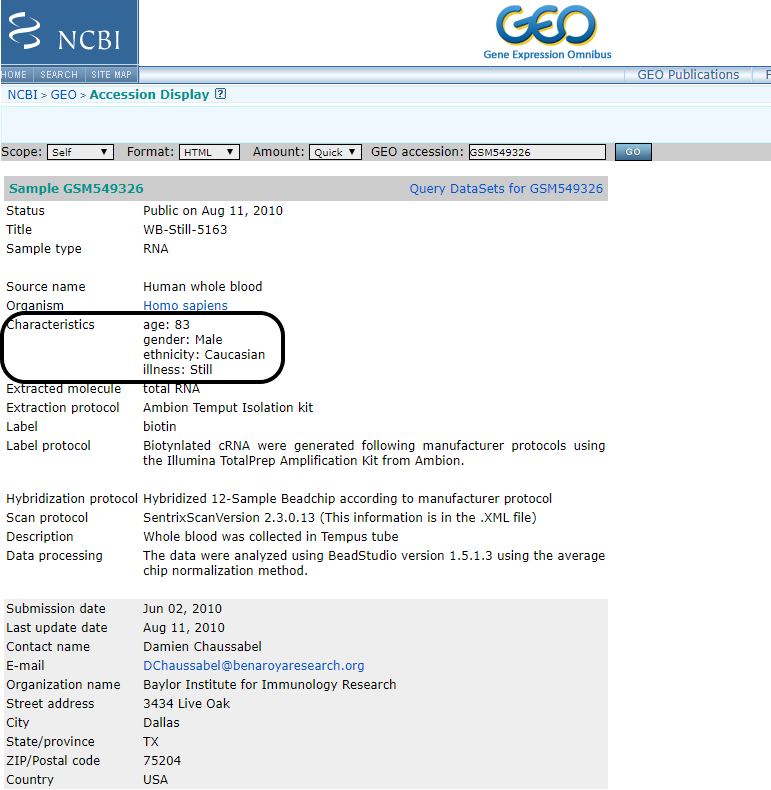
\includegraphics[scale=0.5]{Figures/sample.png}
\caption{An example of GEO Sample}
\label{figure: sample}
\end{figure}
The highlighted part is the field characteristics. The field is structured as key: value pairs where ``age'' is the key and the number $83$ is the value. We chose the ``characteristics'' field since it is semi-structured.
Examples of good metadata and bad metadata in presented in Figure~\ref{fig:bad_meadata} and~\ref{fig:biosample}. From the Figure~\ref{fig:bad_meadata}, in the field about gender it is filled with the number $2$ - which is semantically inaccurate as it is unclear what the 2 refers to. Thus it is difficult to understand what that Sample was about. Similarly, there is no way a human being lives for 160 years, but in the metadata \emph{age: 160} is mentioned. If someone wants to understand what this information is about except that it is something about human beings, it would not be a very trivial task. On the other hand, from the Figure~\ref{fig:biosample}, one can make out the experiments involved human beings and about leukemia.

\begin{figure}[ht]
    \centering
    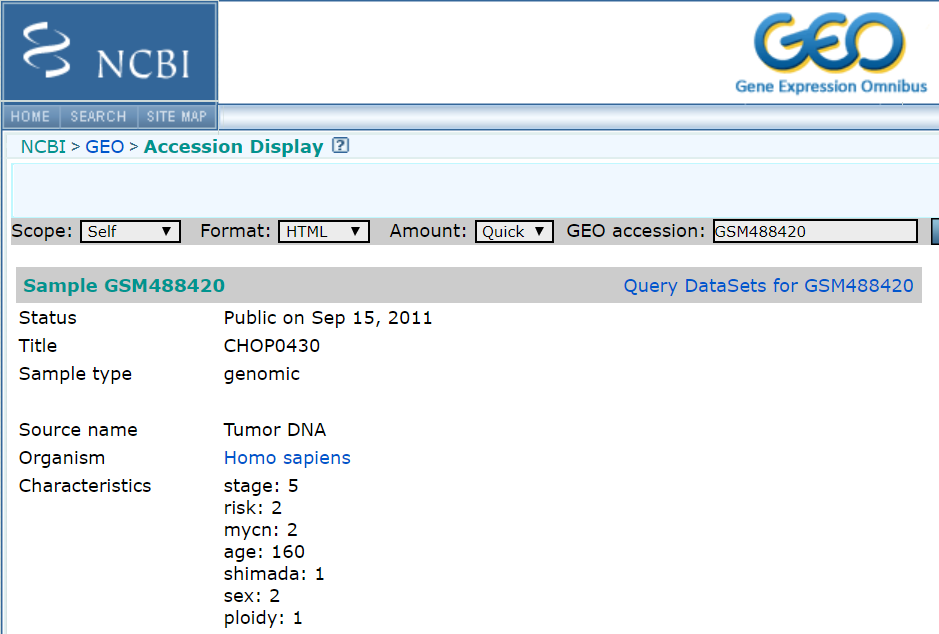
\includegraphics[scale=0.5]{Figures/Capture_geo.png}
    \caption{Example of a bad metadata}
    \label{fig:bad_meadata}
\end{figure}

\begin{figure}[ht]
    \centering
    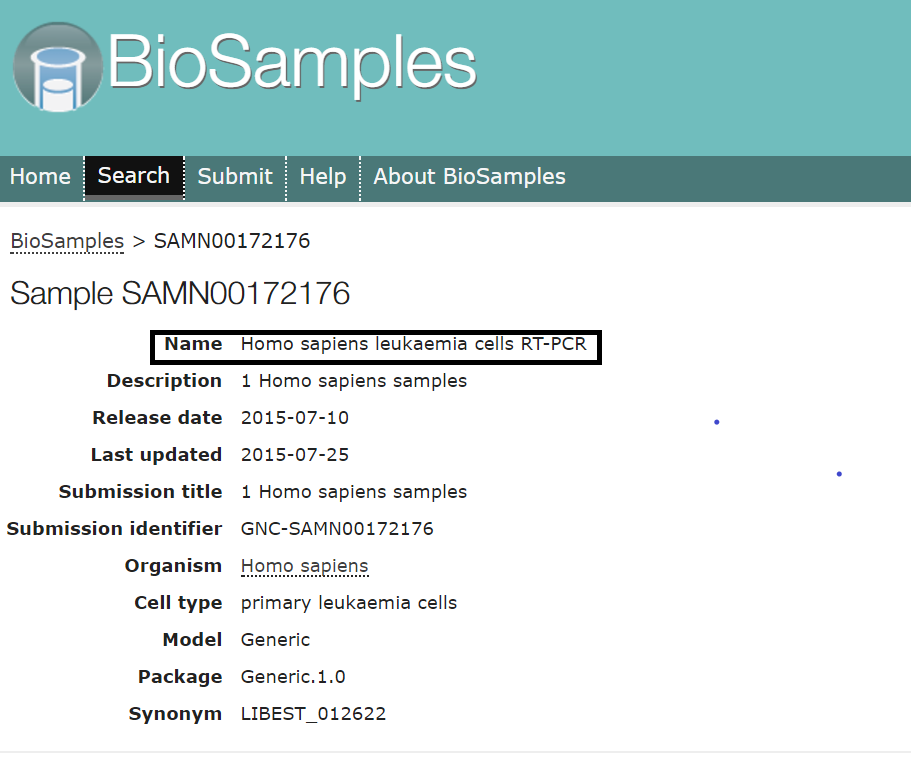
\includegraphics[scale = 0.4]{Figures/Biosamples.png}
    \caption{Example of a satisfactory metadata}
    \label{fig:biosample}
\end{figure}

%\todo{write more about why this dataset and why disease}
The scientific publications contain a lot of information about the experiments done, this information would be useful to determine good metadata. Therefore for predicting metadata, the first step is to look for a gold standard dataset which would have annotated terms of metadata elements. We first start with the metadata category \emph{disease}, for that we need to have a dictionary which can be used for predicting disease values. Therefore, for this purpose, we use the NCBI Disease Corpus~\cite{dougan2014ncbi}. This corpus identifies disease terms using 14 human annotators in 793 scientific publication abstracts and titles from PubMed~\footnote{\url{https://www.ncbi.nlm.nih.gov/pubmed/}}, which serves the purpose as when we test the model with a known scientific text we would know how accurate are the predictions. This corpus identifies disease terms and links it to ontology namely Medical Subject Headings (MeSH)\footnote{\url{https://www.nlm.nih.gov/mesh/}} and Online Mendelian Inheritance in Man (OMIM)\footnote{\url{https://www.omim.org/}}. 

The disease names identified are classified into the following four concepts: 
\begin{itemize}
    \item DiseaseClass: A string which represents a family of diseases, then it was annotated to a disease class. For example: ``autosomal recessive disease'' is a \emph{Disease Class} category.  
    
    \item SpecificDisease: A string that does not have any children class. For example: ``Diastrophic dysplasia'' is a \emph{Specific Disease}. 
    
    \item Modifier: A string that is a disease name but it might modify a sentence containing a noun. In simple words, if a disease name occurs which is a secondary and tries to focus on any other disease is annotated as a \emph{Modifier}. 
    
    For example: In the abstract text ``Although this mutation was initially detected in four of 33 colorectal cancer families analysed from eastern England, more extensive analysis has reduced the frequency to four of 52 English HNPCC kindreds analysed.'' 
    
    The experts are asked to annotate in this way: ``colorectal cancer'' as Modifier category and ``HNPCC'' as Modifier category. 
    
    \item CompositeMention: If more than one disease names occur together then that string was annotated to \emph{Composite Mention}. 
    
    For example, a protein required for ubiquitin-mediated degradation of beta-catenin, but a small percentage of colon and some other cancers harbour beta-catenin-stabilizing mutations. 
    
    The Annotation is - ``colon and some other cancers'': CompositeMention
    
\end{itemize}
 An example of annotation is shown in Listing~\ref{annotation}. 
The number $10192393$ is the PubMed Identifier, the string ``$|$t$|$'' denotes the title and ``$|$a$|$'' denotes the abstract of the scientific publications. All the terms below the abstract are the identified disease terms such as skin tumour, cancer etc. The terms ``D012878'', ``D009369'' are the unique identification number of skin tumour and cancer respectively from the MeSH ontology. 

\begin{lstlisting}[caption=An example of annotation, label=annotation]
10192393|t|A common human skin tumour is caused by activating mutations in beta-catenin.
10192393|a|WNT signaling orchestrates a number of developmental programs. In response to this stimulus, cytoplasmic beta-catenin (encoded by CTNNB1) is stabilized, enabling downstream transcriptional activation by members of the LEF/TCF family. One of the target genes for beta-catenin/TCF encodes c-MYC, explaining why constitutive activation of the WNT pathway can lead to cancer, particularly in the colon. Most colon cancers arise from mutations in the gene encoding adenomatous polyposis coli (APC), a protein required for ubiquitin-mediated degradation of beta-catenin, but a small percentage of colon and some other cancers harbour beta-catenin-stabilizing mutations. Recently, we discovered that transgenic mice expressing an activated beta-catenin are predisposed to developing skin tumours resembling pilomatricomas... 
10192393    15    26    skin tumour    DiseaseClass    D012878
10192393    443    449    cancer    DiseaseClass    D009369
10192393    483    496    colon cancers    DiseaseClass    D003110
10192393    539    565    adenomatous polyposis coli    SpecificDisease    D011125
10192393    567    570    APC    SpecificDisease    D011125

\end{lstlisting}

As mentioned earlier, the corpus contains in total 793 PubMed titles and abstracts which is divided into three sets (i) training, (ii) testing and (iii) development. The Table~\ref{table_ncbi} shows details of the corpus:

\begin{table}[h!]
\caption{NCBI disease Corpus characteristics}
\label{table_ncbi}
\begin{tabular}{|c|c|c|c|}
\hline
\textbf{Corpus Characteristics} & \textbf{Training} & \textbf{Development} & \textbf{Testing} \\ \hline
PubMed Citations                & 593               & 100                  & 100              \\ \hline
Disease Mentions                & 5,148             & 791                  & 961              \\ \hline
Specific Disease                & 2,959             & 409                  & 556              \\ \hline
Disease Class                   & 781               & 127                  & 121              \\ \hline
Modifier                        & 1,292             & 218                  & 264              \\ \hline
Composite Mention               & 116               & 37                   & 20               \\ \hline
\end{tabular}
\end{table}

%As mentioned in Table~\ref{table_ncbi} the corpus contains 793, the Figure shows a word cloud of the abstract text.
The corpus is annotated by fourteen domain experts. There were two-annotators per document which were paired randomly. The annotation was completed in three phases and was checked for consistency throughout the whole corpus as shown in the Figure~\ref{fig:annotationdetails}. In total, we have $2136$ diseases. The statistics of the annotations are as follows are shown in Table~\ref{table: input_stats}. 

\begin{figure}[ht]
    \centering
    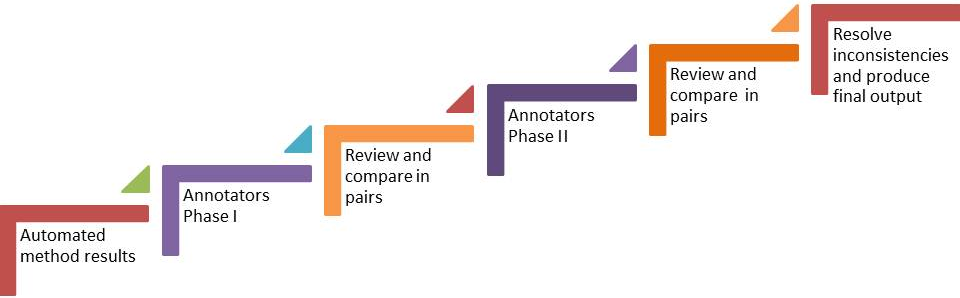
\includegraphics[scale=0.5]{Figures/annotationprocess.png}
    \caption{Annotation Process (Source: \url{https://www.ncbi.nlm.nih.gov/CBBresearch/Dogan/DISEASE/})}
    \label{fig:annotationdetails}
\end{figure}

\begin{table}[ht]
\caption{Input corpus statistics}
\label{table: input_stats}
\centering
\begin{tabular}{|l|l|}
\hline
\textbf{Target Labels} & \textbf{Count} \\ \hline
CompositeMention       & 112            \\ \hline
DiseaseClass           & 571            \\ \hline
Modifer                & 222            \\ \hline
SpecificDisease        & 1231           \\ \hline
\textbf{Grand Total}   & \textbf{2136}  \\ \hline
\end{tabular}
\end{table}


\paragraph{Data Preprocessing}
In the dataset, we have a set of scientific publication titles and abstracts in addition to the identified disease terms and respective disease concepts from the ontology as we saw in the Listing~\ref{annotation}. 
Since a neural network model cannot process raw text data, there is a need to perform some preprocessing stops.
Firstly, the data is cleaned by removing all the (i) punctuation (filters=\verb|’!”#$%&()*+,-./:;<=>?@[\\]^_|), (ii) numbers and (iii) convert all the text into lowercase.  
For training the model, we only use (i) the abstract, (ii) the disease names and (iii) the Unique ID of these diseases from the MeSH ontology. The abstract is used because it contains more information when compared to the title. After that, the text is separated from the disease names as we treat the disease names as the labels that would be identified using the text by the model.
We get the following characteristics of the abstracts:
\begin{itemize}
    \item max length:  450
    \item mean:  191.1640826873385
    \item min length:  32
    \item median:  190.0
\end{itemize}
\paragraph{Text Preprocessing} The text is tokenized - converted into a list of words, and fit according to the size of the text, this converts the text into a set of words which could be called tokens.
Then these tokens are integer encoded - given a unique index, the highest number being the size of the words. 
Then we convert these words into a sequence which gives the words a unique identification number. Then we need to pad this sequence which means to normalize the sequences into a maximum length so that the neural network knows what length of the sequence to expect. 
For example - some sentences will be less than 200 let's say 155, so we insert 45 zeros to make it 200. Some might be bigger say 220, so we remove last 20. We test the model with varying sequence lengths. 

%\paragraph{Label Matrix} To construct a label matrix we need to create a one-hot encoded matrix of the size of the labels we have. In this context, the labels are disease names, for example, if we have 3 diseases the encoded vectors would be in the form of the Table~\ref{table:one_hot}. 

%\begin{table}[ht]
%\caption{Example of one-hot encoding}
%\label{table:one_hot}
%\centering
%\begin{tabular}{|c|c|c|}
%\hline
%\multicolumn{1}{|l|}{disease1} & \multicolumn{1}{l|}{disease2} & \multicolumn{1}{l|}{disease 3} \\ \hline
%1                              & 0                             & 0                         %     \\ \hline
%0                              & 1                             & 0                         %     \\ \hline
%0                              & 0                             & 1                         %     \\ \hline
%\end{tabular}
%\end{table}


%\subsection{Feature Selection}
%For feature selection a Term frequency-inverse document (TF-IDF) approach is used. For each document, a weight is assigned to each term which is essentially the number of times that term occurs in the document (i.e. the frequency of the term.)

%\section{Neural Network Method}
%Chapter~\ref{chap:nnmethod}

\chapter{Methods for Text Classification}\label{chap:nnmethod}

\section{Introduction}

The problem of text classification or text categorization poses the following problem: assign a set of predefined categories to unstructured text that can be used to organize and structure the text appropriately according to the use case. Text classification is an pivotal problem with several applications in biomedicine. For instance, problems such as recognizing reportable cases of cancer from pathology reports, identifying certain phenotypes from clinical notes, performing word sense disambiguation (that is, given a context determine the semantic meaning for the usage of an ambiguous word), and associating medical subject headings (MeSH terms) to scientific articles, can all be reduced to instances of generic text classification problem. Further, text classification can be grouped into two categories namely, (i) multiclass classification (i.e. labels are mutually exclusive) and (ii) multilabel classification where each input can be assigned to more than one label. By definition, it is clear that multiclass classification is a special case of multilabel classification and hence the latter problem becomes more harder to solve than the former.


Traditionally, the problem of text classification is solved by leveraging discriminative models (models that model decision boundary by estimating posterior probabilities) such as support vector machines (SVMs) and logistic regression (LR), only to mention a few, trained on features extracted from the text including bag of words (BOWs)~\cite{sebastiani2005text}. Moreover, it has been observed in the literature that performance gains are achieved with better feature selection techniques, underlying dataset selection, and ensemble approaches~\cite{zhou2012ensemble}. On the other side, better performing models have also be devised by leveraging the field of feature engineering, where the objective is to derive domain specific features that are more relevant and important. For instance, emoticons, exclamations and hashtags form important features for sentiment analysis of Twitter feed~\cite{kiritchenko2014sentiment}. Moreover, especially in the field of biomedicine, exploiting interoperable concept explanations and inter-concept relations from domain specific knowledge base such as unified medical language system (ULMS)\footnote{https://www.nlm.nih.gov/research/umls/} have led performance gains in the accuracy of the underlying models~\cite{yepes2015knowledge}. To this end, models with linear classifiers with ensemble modeling and domain specific feature engineering has the capacity to attain competitive results for the task of text classification.

We perform two experiments for the problem of text classification: (i) Baseline multi-label classification and (ii) Deep learning - specifically CNN and BiLSTM. We illustrate a comparison of the performance of the aforementioned methods in Chapter~\ref{chap: results}. The motivation behind this comparison of employing two techniques is to answer the research question as to which method performs better when we deal with prediction of metadata (Refer RQ4 in Chapter~\ref{chap:intro}).

\section{Baseline Multi-label Classification}\label{MLtranform}
The number of labels (or categories) entails the different kinds of classification problems. For example: if the number of labels $|L| = 2$ then the problem is called binary classification, for $|L| > 2$ labels the problem becomes a multi-class classification. The problem of multi-label classification similarly deals with more than one label, but each label is considered as a different classification problem, but these problems are somewhere related to each other. On the contrary, in a multi-class classification the labels are mutually exclusive~\cite{tsoumakas2007multi}. For instance in a multi-class problem would consider that a scientific publication would only talk about one out of several diseases. Whereas in a multi-label classification the scientific publication might talk about several diseases or none diseases at all. 
In order to use the traditional classification techniques like Random Forest Classifier, Decision trees and so on, the problem needs to be transformed in a way that these techniques can be used. In this project we use three transformation techniques (i) Binary Relevance, (ii) Label Powerset and (iii) Classifier Chains. 
\subsection{Problem Transformations}
Here we briefly describe the problem transformations where traditional classification techniques are modified in such a way that they can be used to perform multi-label classification. 
\paragraph{Binary Relevance (BR)} 
This transformation converts the multi-label problem into a single label problem for each label. Once these problems are solved, a union is taken for all the classes which is the output of the problem. In simpler words, this problem solves a binary classification for each label with any classifier picked as seen in Figure~\ref{fig:BR}. The major disadvantage in this approach is that it does not take label dependencies into account. 
\begin{figure}[!htb]
    \centering
    
\includegraphics[scale=0.5]{Figures/BinaryRelevance.png}
    \caption{Multi-label problem transformation - Binary Relevance}
    \label{fig:BR}
\end{figure}

\paragraph{Label Powerset (LP)} 
In this problem transformation, a multi-label problem is converted into a single multi-class problem which can take many values. It takes the labels $y_1, y_2, ...., y_n$ (refer Figure~\ref{fig:LP}) and makes several combinations of these labels and solves a multi-class problem for every such combination. This method computes a large space of classes. In total it solves $2^{|L|}$ such problems where $|L|$ is the number of labels. 
\begin{figure}[!htb]
    \centering
    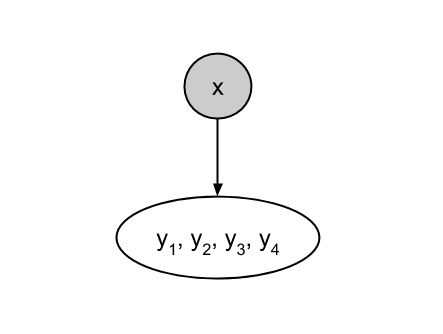
\includegraphics[scale=0.5]{Figures/LabelPowerset.png}
    \caption{Multi-label problem transformation - Label Powerset}
    \label{fig:LP}
\end{figure}

\paragraph{Classifier Chains (CC)}
Classifier chains~\cite{dembczynski2010bayes, read2011classifier} are an improvement in the BR transformation, which takes into account the dependency between the labels if there exists any. Let's say the feature set is: ($x_1, x_2, x_3,....., x_n$) and the set of labels is: ($y_1, y_2, y_3,\ldots, y_n$). The initial feature set is used to predict $y_1$, after that ($x_1, x_2, x_3,\ldots, x_n, y_1$) is used to predict $y_2$. At $n^{th}$ step, feature set ($x_1, x_2, x_3,\ldots, x_n, y_1, y_2, y_3,\ldots, y_{n-1} $) predicts $y_n$ (refer Figure~\ref{fig:CC}). The order of prediction can be tuned in order to get better results. For a large set of labels this method is slow as it takes $n!$ combinations of orderings. 
\begin{figure}[!htb]
    \centering
    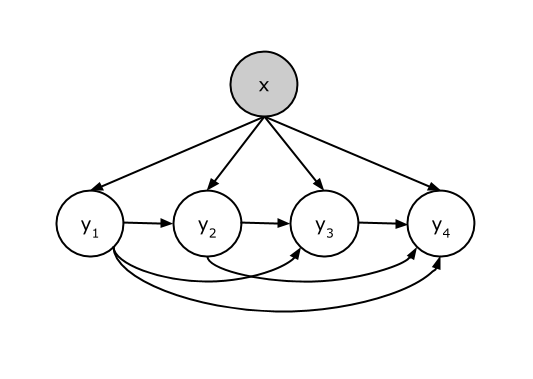
\includegraphics[scale=0.5]{Figures/ClassifierChains.png}
    \caption{Multi-label problem transformation - Classifier Chains}
    \label{fig:CC}
\end{figure}

\subsection{Problem adaptation and Classifiers}
Here we discuss about the adaptation of existing classification algorithms so that they have the ability to perform multi-label classification. Furthermore, we discuss the standard classifiers that have been used. 

\paragraph{Multi-label k Nearest Neighbours (MLkNN)} 
Another adaptation of k nearest neighbours(kNN) for multi-label classification was done by~\cite{zhang2007ml}. In kNN assigns the most commonly occurring neighbours among the calculated k `nearest neighbours'. Whereas in MLkNN, the labels assigned are the most common labels in the neighbourhood of k nearest neighbours. In simpler terms, given a test set, MLkNN uses kNN to find nearest examples and uses Bayesian Inference to predict the labels.

\begin{equation}
 y_{j} = 
\begin{cases}
    1, & \text{if } P(c_{j,x}|y_j = 1)P(y_j = 1) \geq P(c_{j,x}|y_j = 0)P(y_j = 0) \\
    0, & \text{otherwise}
\end{cases}
\end{equation}

(where $c_{j,x} :=$ the number of number of examples present in the neighbourhood of $x$ with $y_j = 1$; Probabilities calculated from the training data)

\paragraph{Decision Trees (DT)}
A decision tree use tree structure perform classification. In such a tree (i) each interior node tests one attribute, (ii) every branch corresponds to an attribute and (iii) each leaf node is the labelled with the class i.e. label/category. A classification using decision tree is presented in Listing~\ref{DT}. It is a strategy for approximating discrete-esteemed capacities that is powerful to load information and equipped for learning disjunctive expressions. The group of decision tree learning calculation incorporates generally utilized calculation, for example, ID3~\cite{quinlan1986induction}, CART~\cite{breiman2017classification} and C4.5~\cite{xiaoliang2009research}. These decision tree learning techniques seek totally expressive speculation space and hence keep away from the troubles of limited theory spaces. Their inductive inclination is an inclination for little trees over substantial trees. 
\begin{lstlisting}[caption = Classification with Decision Trees, label = DT]
Classify(x: instance, node: variable containing a node of DT)
    if node is a classification node then
        return the class of node;
    else
        determine the child of node that match x.
        return Classify(x, child).

\end{lstlisting}



%\todo{still to add brief description about random forest and MLP}
\paragraph{Random Forest}
A random forest is an information build connected to machine learning that grows substantial quantities of random decision trees dissecting sets of factors~\cite{breiman2001random}. This sort of calculation improves the manners in which that advances examine complex information. 

All in all, decision trees are famous for machine learning assignments. In a random forest, engineers build sets of random decision trees to all the more cautiously detach information from information mining, with various connected variable exhibits. One approach to portray the theory behind the random forest is that since the random trees have some cover, specialists can assemble frameworks to consider information needlessly with the different trees and search for patterns and examples that help a given information result. For instance, if five random trees give data on a similar variable from a subset, and four of them concur, the machine learning calculation may use that "dominant part vote" to construct models dependent on probabilities. In a wide range of sorts of machine learning, develops like the random forest can assist mechanical frameworks with drilling down into information and give increasingly modern investigation.

\paragraph{Multi-layer perceptron (MLP)}
Although neural networks are also explained in Section~\ref{section:architecture}, we define MLP here as we use it as a baseline classifier. 
Multilayer feed forward networks, an essential class of neural networks~\cite{haykin1994neural}. Typically, the system comprises of a lot of tangible unit (source hubs) that establish the info layer, one or increasingly concealed layers of computational nodes, and a yield layer of calculation nodes. The input flag engenders through the system in a forward direction, on a layer-by-layer basis. These neural systems are regularly alluded to as multilayer perceptrons (MLPs), which speak to a speculation of the single-layer perceptron. 

Multilayer perceptrons have been connected effectively to tackle some troublesome and differing issues via preparing them in an administered way with a profoundly prominent calculation known as back-engendering calculation. 
A multilayer perceptron has three particular qualities: 
\begin{enumerate}
    \item The model of every neuron in the system incorporates a nonlinear enactment work. 

    \item The system comprise of at least one layers of concealed neurons that are not part of the information or yield of the network. These shrouded neurons empower the system to learn complex assignments by separating dynamically progressively significant highlights from the information design. 

    \item The system displays high degrees of connectivity, determined by the neural connections of the system. 
\end{enumerate}
It is through the mixture of these attributes together with the capacity to gain as a matter of fact through preparing that the multilayer perceptron determines its registering power.

\section{Deep Learning}
The advent of deep neural networks (deep nets) in the last decade or so has led to foundation for generic alternatives to supervised learning, especially for the task of object classification. Deep nets eliminate the laborious process of feature engineering and automatically learn high level representations of input which suites best for the underlying classification problem. Although, the resurgence of deep nets was initially meant for the field of computer vision, recently it has also been applied to natural language processing tasks (NLP)\cite{bengio2003neural, collobert2008unified, mikolov2013distributed} especially through learning distributed representations of words as vectors in high dimensional space. These vectors help the model in guiding elementary tasks such as part-of-speech (POS) tagging and parsing as well as abstract tasks such as text classification and machine translation. Typically, the novel deep learning approaches for text classification rely on architectures based on convolutional neural networks (CNNs) or recurrent neural networks (RNNs)~\cite{young2018recent}. In Figure \ref{fig:dlarch}, you can see a typical deep learning based text classification architecture pipeline.


% . For instance, scientific articles can be filtered by keywords, support tickets can be organized by urgency, tweets on twitter can be organized by sentiments, and so on. Due to the advent of deep learning in the last decade and especially their potential to attain high accuracies has benefited the task of text classification unconditionally. 



\begin{figure}[!htb]
    \centering
    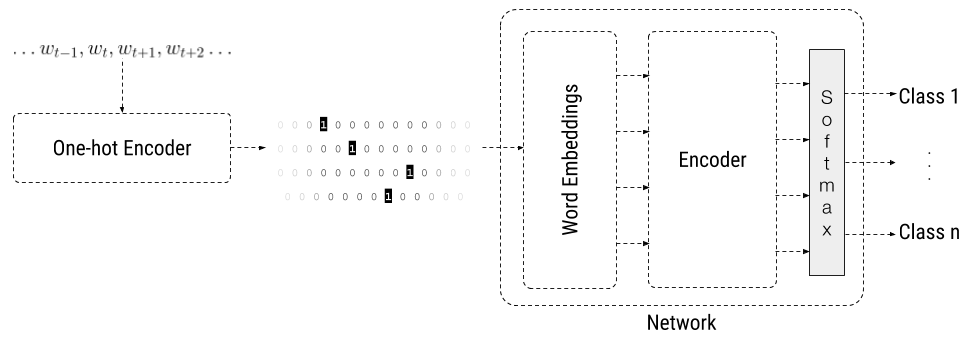
\includegraphics[scale=0.4]{Figures/text-classification-diagram.png}
    \caption{Typical neural network based deep learning architecture for multiclass classification of texts.}
    \label{fig:dlarch}
\end{figure}


Now we unfold each and every component of the architecture in Figure \ref{fig:dlarch}. 

\subsection{Unfolding the architecture}\label{section:architecture}

For an average human, understanding the inherent meaning of the words based on the context they are used, is an easy task. In the same spirit, a deep learning model needs a clever representation of text segments so that it can understand the semantic similarity of related words and also differentiate each word from others. 


\paragraph{One-hot Encoding} Assigning unique, discrete IDs to the word tokens, that is, represented by a \emph{one-hot encoding vector} helps in understanding the model to differentiate between two different words. This in turn has an advantage as neural networks expect vectors as input. Although, this still does not provide any useful information to the model about the relationship between the words and in fact additionally, leads to \emph{sparsity}. 
% This entails that we may need more data in order to obtain meaningful statistical results. 
To state an example, treating words as discrete atomic symbols, for instance, representing a \emph{cat} by \emph{Id100} and \emph{dog} by \emph{Id150} does not provide any meaningful information to the model regarding the relationship that may exist between the two symbols as they are some arbitrary encodings. This amounts to the model leveraging very little of what it has learned about \emph{cats} when it is processing data about \emph{dogs} (such that they are both animals, four-legged, pets, only to mention a few).

\paragraph{Word Embeddings} To overcome the problems regarding sparsity and semantic similarity of related words in one-hot encoding,~\cite{bengio2003neural} developed the concept of word embeddings back in 2003. Despite being introduced before, word embeddings are still relevant today and highly active research domain in deep learning~\cite{bojanowski2017enriching, joulin2017bag, joulin2016fasttext, Peters:2018}. The concept relies on the \emph{Distributional Hypothesis} of J.R. Firth (1957) that states that \emph{``You shall know a word by the company it keeps"}, that is, words that appear in the same contexts share semantic meaning. As we are in the context of neural networks, we are only concerned with predictive methods (i.e. neural probabilistic language models). Predictive models directly try to predict a word from its neighbors in terms of learned small, dense embedding vectors (considered parameters of the model).



A word embedding $\mathcal{W} : \text{words} \rightarrow \mathbb{R}^n$ is a parameterized function that maps words to high dimensional vectors (typically between 200 to 500 dimensions). In other words, it is a dense vector space that forces a fixed dimension on the vector space and forces similar words to appear nearby each other across some dimensions. Typically, the function $\mathcal{W}$ is a look-up table, parameterized by a matrix $\theta$ where each row corresponds to an embedding for a particular word: $\mathcal{W}_{\theta} (w_n) = \theta_n$ (refer Figure \ref{fig:word-embedding-matrix}). $\mathcal{W}$ is initialized randomly by having random row vectors for each word and the model learns to capture meaningful syntactic and semantic regularities in order to perform some task. Word2vec~\cite{mikolov2013distributed} and GloVe~\cite{pennington2014glove} are the two most popular word embedding models to obtain off-the-shelf trainable word embedding matrices. Moreover, word embeddings exhibit an interesting property, namely, it encodes semantic components as linear vector differences. (refer Figure \ref{fig:linear-vector}). 
 

\begin{figure}[!htb]
    \centering
    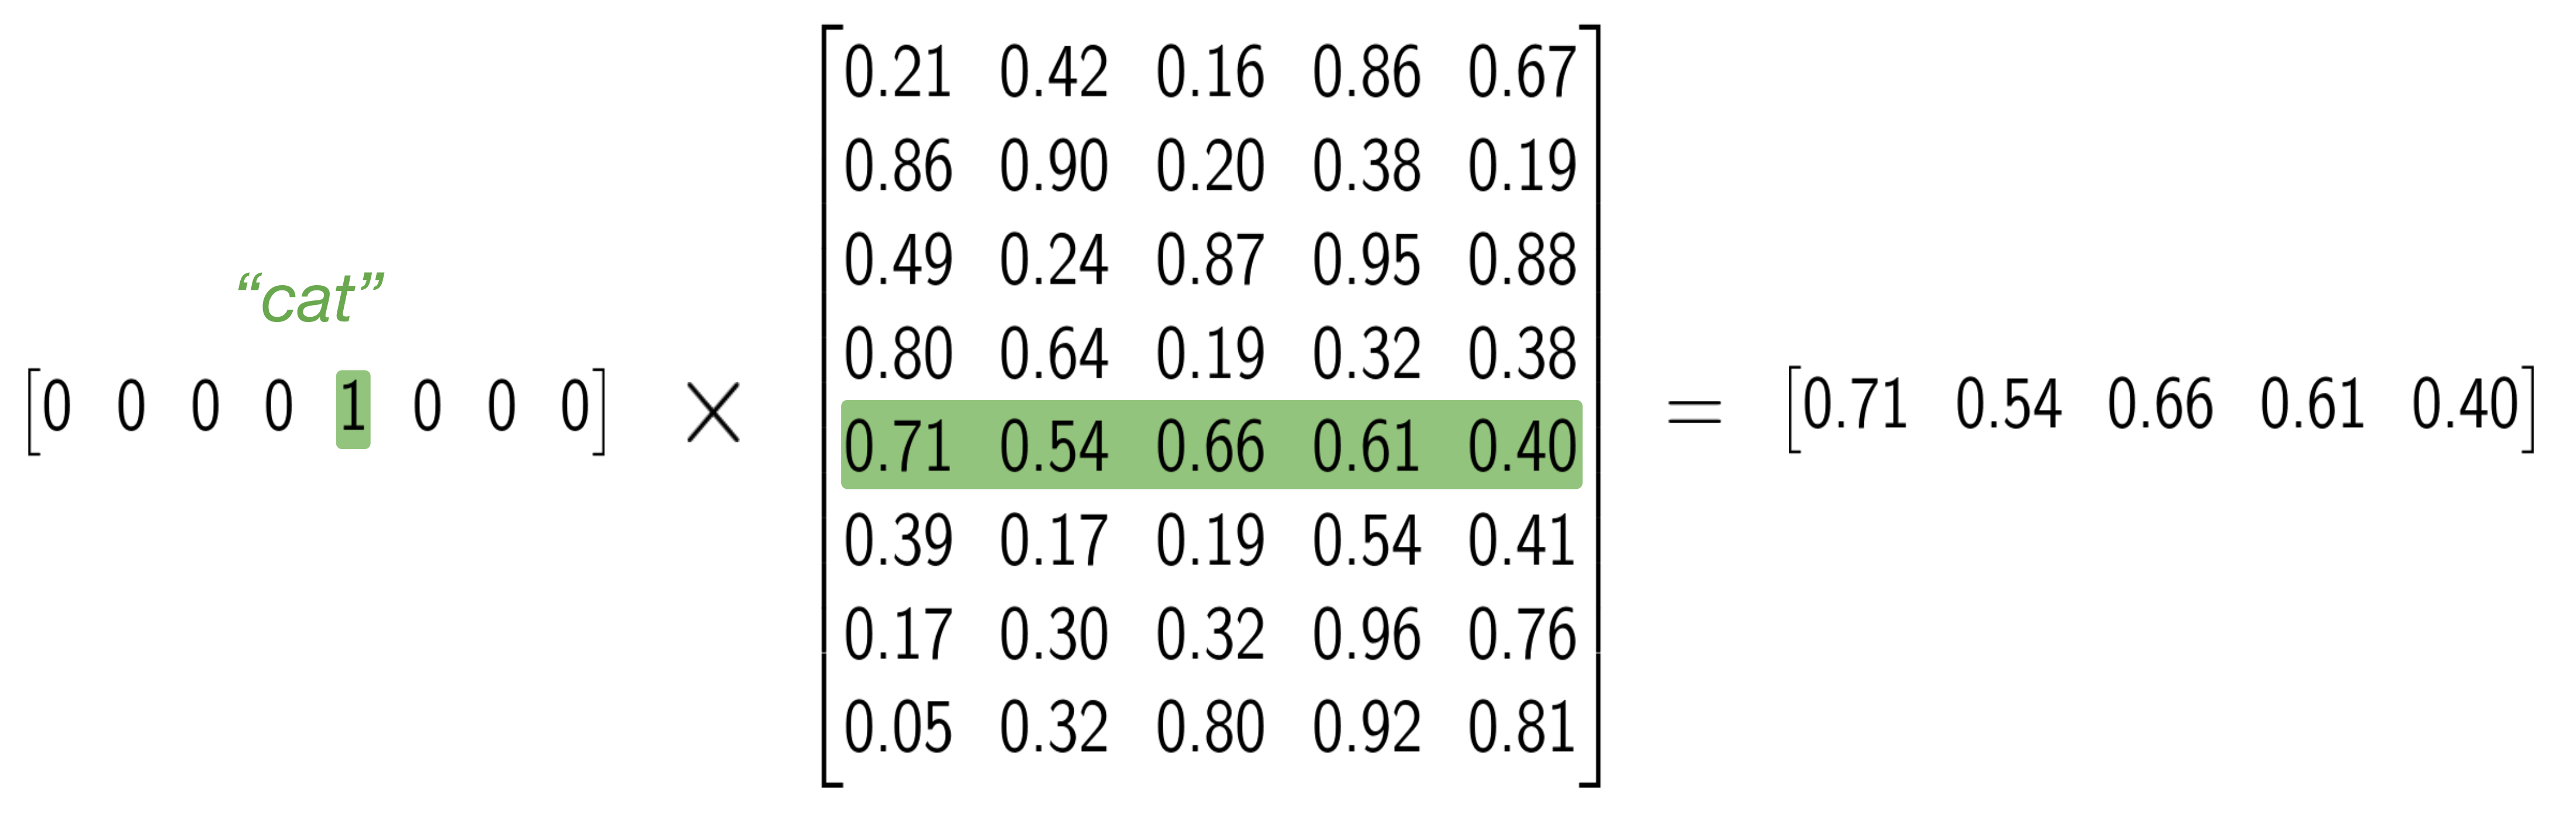
\includegraphics[scale=0.5]{Figures/word-embedding-matrix.png}
    \caption{The figure illustrates how to obtain embedding of a particular word \emph{``cat"} from a word embedding matrix. The one-hot encoding vector of the word \emph{``cat"} is multiplied to the word embedding matrix to obtain the embedding vector for \emph{cat}.}
    \label{fig:word-embedding-matrix}
\end{figure}


\begin{figure}[!htb]
    \centering
    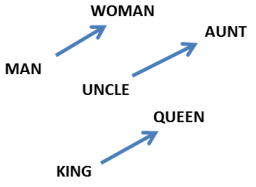
\includegraphics[scale=0.5]{Figures/Mikolov-GenderVecs.png}
    \caption{This figure illustrates the property of word embeddings where linear vector differences between male-female vector is preserved, that is, constant. That is, $\mathcal{W}(``\text{woman}") - \mathcal{W}(``\text{man}") \simeq \mathcal{W}(``\text{aunt}") - \mathcal{W}(``\text{uncle}") \simeq \mathcal{W}(``\text{queen}") - \mathcal{W}(``\text{king}")$ (Image Source~\cite{mikolov2013distributed}).}
    \label{fig:linear-vector}
\end{figure}


\paragraph{Encoder} Once we have the word embedding matrices from the raw text, in order to perform classification tasks, commonly used encoder architectures are convolutional neural networks (CNN) and recurrent neural networks (RNN). Next, we briefly summarize how is the classification task performed using the aforementioned architectures.

\paragraph{Neural Networks}
The neural network (NN) approach is widely used in the machine learning and deep learning algorithms to solve problems with complex, sparse data~\cite{lecun2015deep}. The word `neural' is used because they are loosely inspired by neuroscience. 
%Neural networks are referred to deep feedforward networks or feedforward neural networks.
The goal of such a network is to estimate a function $f^*$.  In a traditional classifier $ y = f^*(\textbf{x})$, it maps the input $\textbf{x}$ to output category $y$. Whereas in the feedforward neural network the model defines a mapping $ y = f(x;\theta)$. It then learns the entries of parameter in $\theta$ which is in-turn best approximation of the function. 
The basic computational unit of a NN is a neuron (refer Figure~\ref{fig:neuron}) which is often referred to as a node or a unit. It receives input from other units or from external source after which it computes an output (see Figure~\ref{fig:vectorinputs}).
\begin{figure}[!htb]
    \centering
    
\includegraphics[scale=0.6]{Figures/neuron.png}
    \caption{Typical neuron in a neural network, which can be intuitively thought of a building block of the underlying neural network.}
    \label{fig:neuron}
\end{figure}
\begin{figure}[!htb]
    \centering
    
\includegraphics[scale=0.6]{Figures/Vector-Inputs-to-Neuron.png}
    \caption{Vector inputs in the neuron}
    \label{fig:vectorinputs}
\end{figure}
%\todo{include weight vector W in figure}
Each output from this neuron consists of an associated weight ($w$), which is calculated according to the relative importance with respect to other inputs. The node applies a weighted function to the sum of inputs.

The intention behind the network is to learn these set of weights and to be able to control the strength and the influence of these parameters according to the problem that is being solved using the NN approach. We control such an effect of the parameters using an activation function which should be associated to a neuron. Using this function, the node computes the output given a set of inputs. One such activation function is Sigmoid: $\sigma(x) = \frac{1}{1+e^{-x}}$. A parameterized sigmoid function is $\sigma_{w,b}(x) = \frac{1}{1+e^{-wx+b}}$. The advantage of using a non-linear activation function such as sigmoid is that these networks are able to solve non-trivial problems using a relatively smaller number of parameters. 
There are also other types of non-linear activation functions such as: hyperbolic tangent  ($tanh$), Rectified Linear Unit($ReLU$). 

%One limitation of the linear classification like linear regression or logistic regression is that it is not able to detect any correlation between two input variables. NNs are used to perform non-linear classification tasks, 
%For example gradient descent which is a derivative of a linear function gives a smooth function, as nonlinear functions are a generalization of linear functions, 
%see clearly in Figure~\ref{fig:linearclassification} and~\ref{fig:nonlinearclassification}. The neural network which uses a sigmoid function as their activation to perform computations $\sigma(x) = \frac{1}{1+e^{-x}}$, similarly a parameterized sigmoid function is: $\sigma_{w,b}(x) = \frac{1}{1+e^{-wx+b}}$ is shown in Figure~\ref{fig:neuron}. The inputs are given in the form of vectors (refer Figure~\ref{fig:vectorinputs}), if the network contains more than one layers, the composite functions are used to calculate the outputs. Other functions than sigmoid as activation like hyperbolic tangent  ($tanh$), Rectified Linear Unit($ReLU$) etc. 
% \begin{figure}[!htb]
%     \centering
%     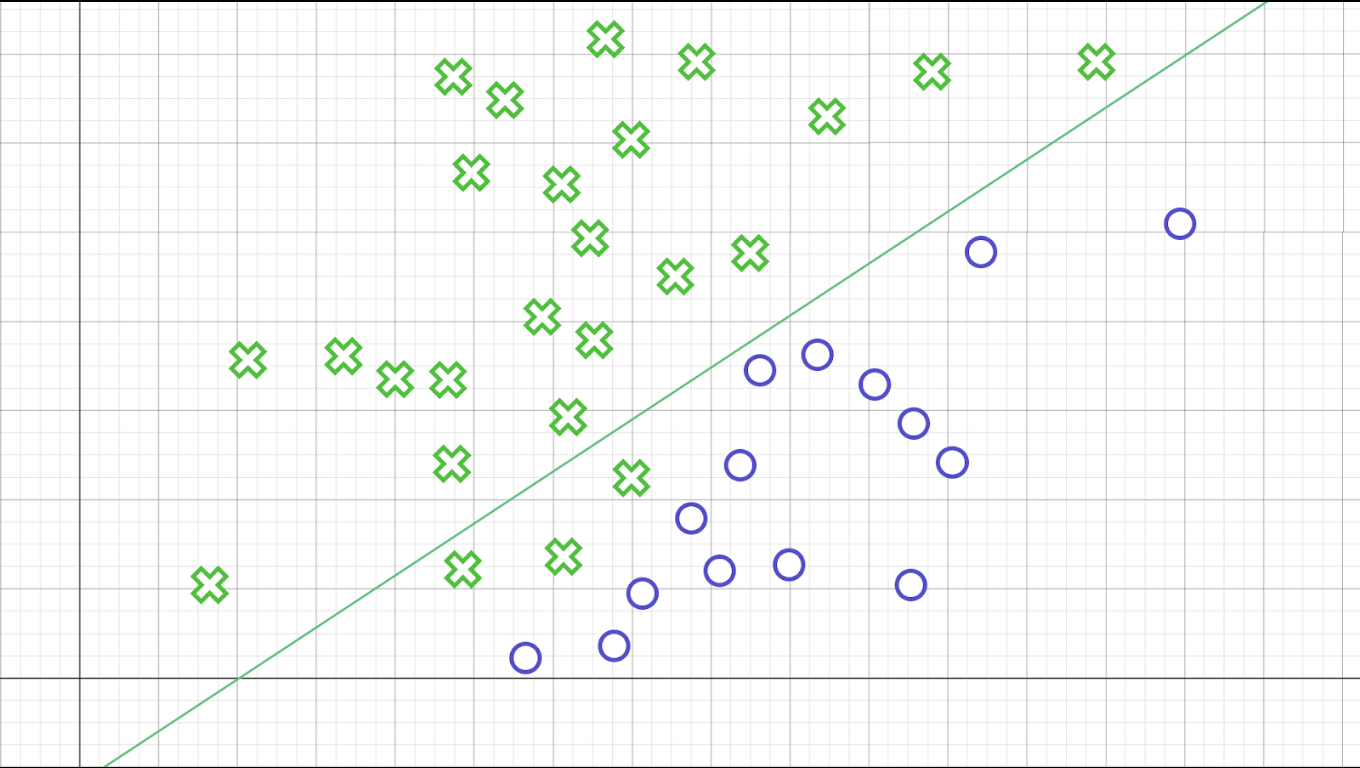
\includegraphics[scale=0.2]{Figures/non-linear_classification.png}
%     \caption{A Linear Classification}
%     \label{fig:linearclassification}
% \end{figure}
% \begin{figure}[!htb]
%     \centering
%     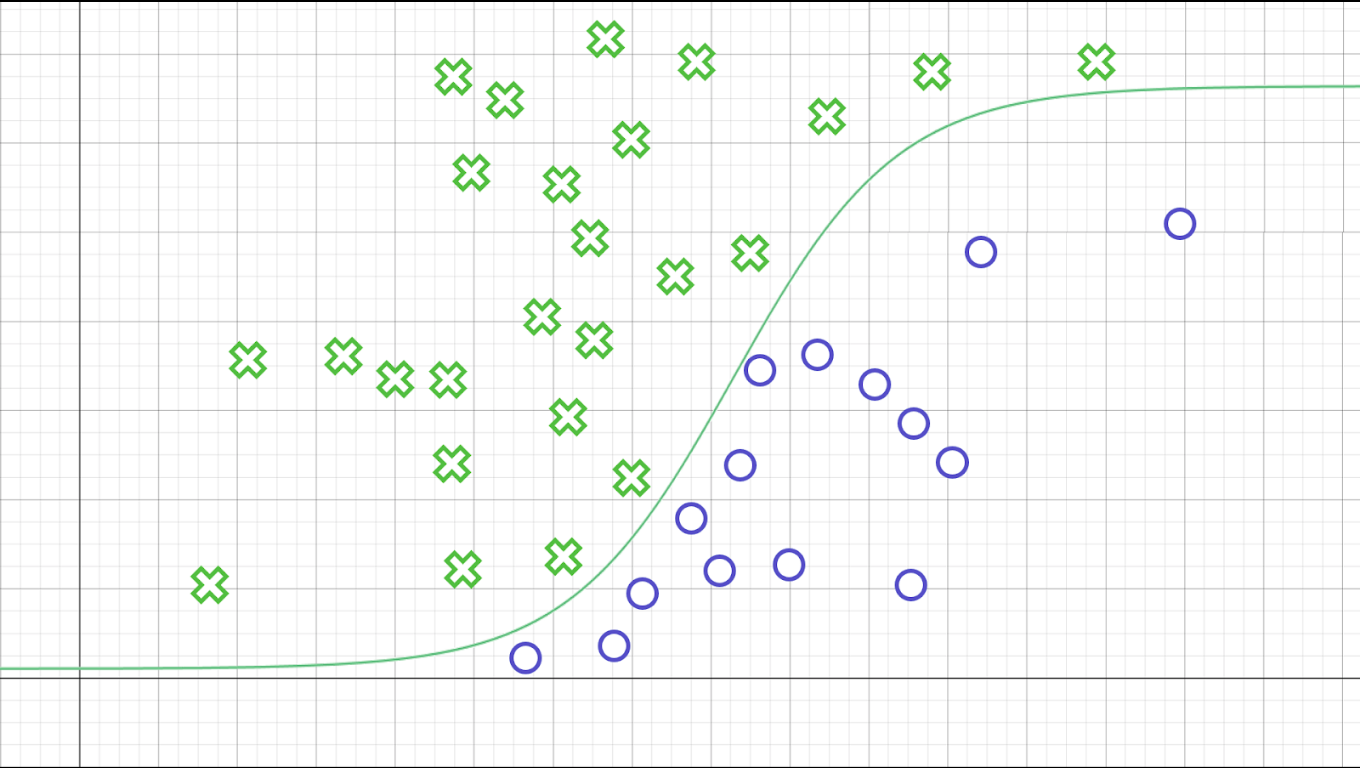
\includegraphics[scale=0.2]{Figures/linear_classification.png}
%     \caption{A Non-linear Classification}
%     \label{fig:nonlinearclassification}
% \end{figure}

In a neural network architecture there are layers which are classified into three type which are mentioned below, all these layers contain nodes which are interconnected to each other in a dense manner also shown in Figure~\ref{fig:nn}:
\begin{itemize}
    \item \textbf{input layer} - this brings in the data into the architecture which is then pass on to the next layer for processing
    \item \textbf{hidden layer(s)} - after the input layers there are a certain number of interconnected layers these can be specified accordingly. Here, the network takes a bunch of weighted set and use an activation function to emit the output.
    \item \textbf{output layer} - last layer of nodes where we get the output.
\end{itemize}
\begin{figure}[!htb]
    \centering
    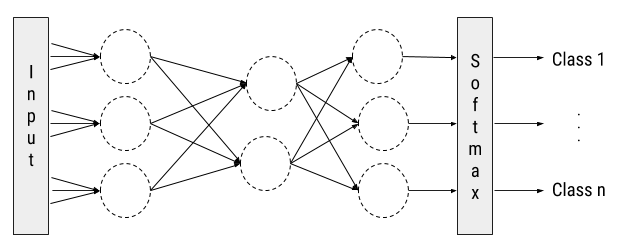
\includegraphics[scale=0.6]{Figures/neural-network.png}
    \caption{A simple neural network architecture for the task of multiclass classification, where the output layer is followed by a softmax layer, that takes outputs from the output layer and converts a distribution of numbers into probabilities.}
    \label{fig:nn}
\end{figure}

While training the neural networks we need to see how every parameter effects on the performance. For this purpose, we calculate the model performance using the function known to us as \emph{loss function}. A loss function is the difference between the model output ($\hat{Y}$) and the given label (Y) for a data point. For instance, one such loss function is mean square error method and is written as, 
\begin{equation}
    L(\hat{Y},Y) = \frac{1}{2n}\sum_{i=1}^{n}(\hat{y}-y)^2
\end{equation}
Given enough hidden units (neurons), a two layered neural network that can approximately imitate any continuous function, over a wide range of activation functions. Although the challenge is to find right values of the parameters given the input data. This is where backpropagation comes into practice. 
We know from high school calculus that for a function $y = f(x)$, $f'(x)$ or $\frac{dy}{dx}$ is an indicative of modifying the value of $x$, where the objective is to minimize $y = f(x)$. That is, in order to reduce $f(x)$, we have to modify $x$ in small steps with an opposite direction of the sign of $f'(x)$--this is gradient descent. Backpropagation is done using gradient descent. The gradients are calculated w.r.t. model parameters for each parameter. The parameters are modified in such a way that the parameters point in that direction where loss is decreasing. The parameters (weights) are modified using the following formulation, where $\eta$ (positive scalar) is a hyperparameter known as learning rate of the neural network model (determines how big a step to take in the direction opposite to the gradient)
\begin{equation}
    w_{n}^{(t+1)} = w_{n}^{(t)} - \eta\frac{dL}{dw_{n}^{(t)}}
    \label{eq:parameterupdate}
\end{equation}

Summarizing from Figure~\ref{fig:oneepoch}, we give the input data $x$ to the neural network, $y$ is the input label of the data and $f_W(x)$ is the model which gives the output $\hat{y}$ ($\hat{y} = f_W(x)$). After this loss is calculated: $L(\hat{y}, y)$. This is the forward propagation. 
Now in the backward  propagation: we calculate gradients $\frac{dL}{dW_{1:n}}$. Then the parameters are updated using the Equation~\ref{eq:parameterupdate} in each epoch. 

\begin{figure}
    \centering
    
\includegraphics[scale=0.5]{Figures/back-propagation.png}
    \caption{A forward and backward propagation in the neural network.}
    \label{fig:oneepoch}
\end{figure}


\subsubsection{CNN}\label{sec:cnn}
Convolutional neural networks are a special kind of neural networks which employ a grid-like operation. The name ``convolution'' is used because it uses the mathematical operation convolution. In simple words: in a CNN convolution operation is used in at least one of the layers in place of general matrix multiplication~\cite{Goodfellow-et-al-2016}.
They are widely used in the context of images~\cite{krizhevsky2012imagenet} where images are consider 2-D grid of pixels. Although, the architecture can be used if sentences or paragraphs or documents can be represented as matrices or vectors, as it is the case in images. Word embedding matrices typically act as pixel matrices of images in the context of text classification. One of the reasons as to why CNNs are successful is because of its inherent property of keeping a number of copies of the same type of neurons. 
%This helps the model to have numerous neurons, while being able to process large complex models keeping same number of parameters. While writing programs in computer science we tend to write a function and keep calling it later on, the CNNs do a similar thing with the help of these large number of neurons. This in turn makes learning easier and reduces error. 
CNN has been successfully applied in NLP tasks~\cite{dos2014deep, zeng2014relation}. 

From the network point of view, CNN's are essentially several layers of convolutions (refer Figure~\ref{fig:CNN_layer}) stacked upon each other with non-linear activation functions applied to the output of neurons in the same layer. 
\begin{figure}[!htb]
    \centering
    
\includegraphics[scale=0.5]{Figures/cnn.png}
    \caption{The figure illustrates the components of a typical convolutional neural network (CNN). The figure in the left views CNN as small number of complex layers, where within each layer a number of operations are applied. While on the right, CNN is viewed as a larger number of simple layers performing elementary operations.}
    \label{fig:CNN_layer}
\end{figure}
A typical layer in a CNN has three stages: (i) convolution operation (refer Figure~\ref{fig:convolution}), (ii) a non-linear activation like rectified linear unit and (iii) a pooling function which lists the set of output with certain statistical explanation of outputs of neighbourhood. These three stages accommodate in the standard feed-forward architecture of linear and non-linear activations. As we can see from Figure~\ref{fig:CNN_layer},
the first stage is linear and the second layer when combined with the third stage form a non-linear activation. 
One of the most used pooling statistics is \emph{max-pooling}. Most commonly, max-pooling is used as a downsampling technique with for instance, say $2 \times 2$ dimension filter and stride equal to 2 , (Figure~\ref{fig:maxpool}), which reduces the representation size and decreases computational and statistical burden on the next layers.



\begin{figure}[!htb]
    % \centering
    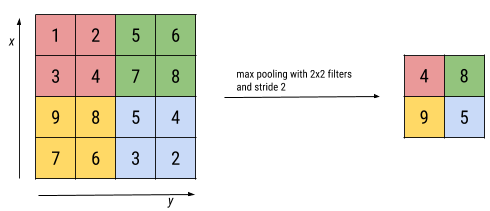
\includegraphics[width=0.6\textwidth, center]{Figures/max-pooling.png}
    \caption{This figure illustrates the operation of max-pooling to summarize the feature maps.}
    \label{fig:maxpool}
\end{figure}
Figure~\ref{fig:convolution} illustrates that convolution is a binary operation that involves two operands namely, some text and a predefined kernel or filter, both of which are represented as matrices containing real numbers.
\begin{figure}[!htb]
    % \centering
    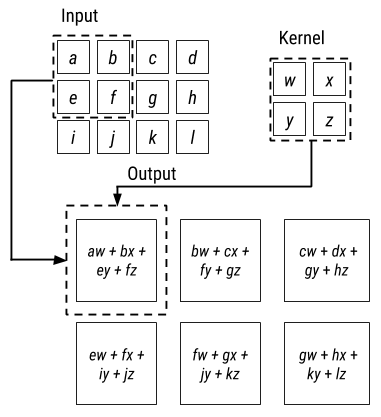
\includegraphics[width=0.6\textwidth, center]{Figures/convolution.png}
    \caption{This figure illustrates the operation of convolution on a 2D image. Boxes and arrows are drawn which indicate how the convolution takes place when the kernel/filter is applied to the upper-left region of the input.}
    \label{fig:convolution}
\end{figure}
Typically, the matrix representation of text comprises of the word vectors of tokens that constitute it, that is, the word embedding matrix. The objective of the kernel is to operate on all contiguous segments of the text using a sliding window and produce real numbers of cardinality that is equal to the number of contiguous segments (in text). This sequence of real numbers is called a feature map and is associated with a particular kernel being used to compute it. Generally, different kernels produce different feature maps that can be used as features for the task of text classification. The feature maps are then fed into a non-linear activation function as input, typically, softmax (function that takes $l$ real values as input and normalizes it into a probability distribution consisting of $l$ probabilities)   in our use case that outputs class or label probability estimates. The main idea here is to learn the matrix representations of kernels that in turn provide better feature maps, which optimizes the objective function efficiently. The learning takes place by predicting labels for training data and make adequate modifications to the kernel matrix through the back propagation algorithm that minimizes the loss function, that is, minimizes the conditional log-likelihood of training data. In the aforementioned abstract elucidation, we have omitted the technical details pertaining to CNNs like mathematical definition of convolution, the objective function and regularization. For the sake of completeness, we discuss these points in detail in the next section.

\paragraph{CNN Model Description}
The architecture of a CNN model with two layers including one convolution layer and a densely connected output layer is depicted in Figure~\ref{fig:Cnn_one_layer}.
\begin{figure}[!htb]
    % \centering
    % 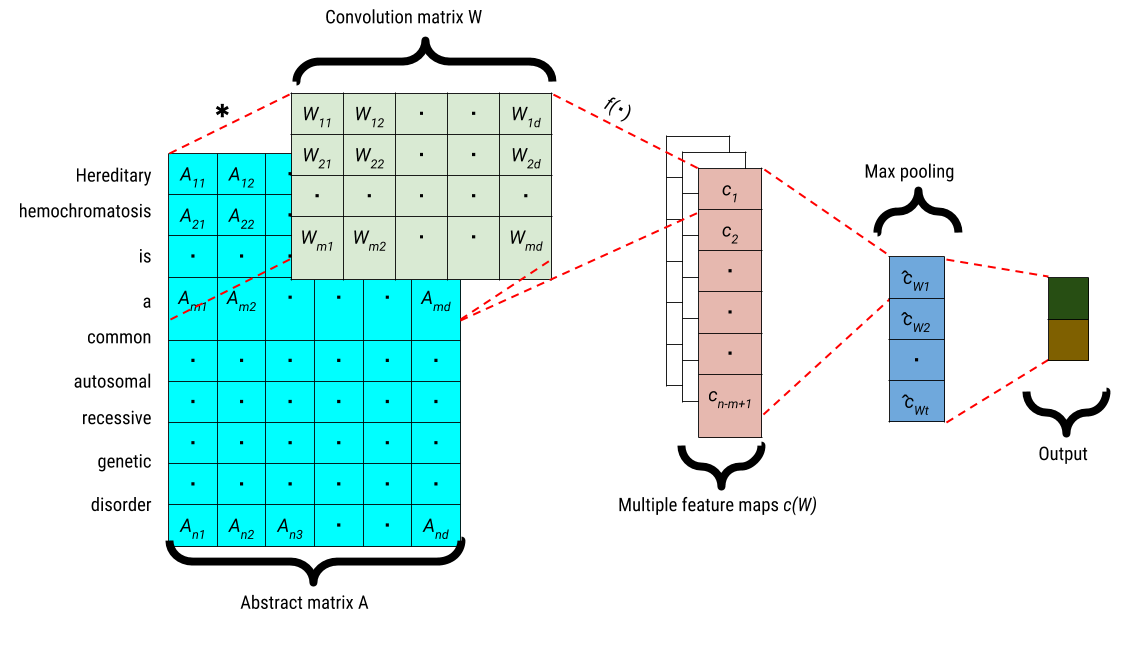
\includegraphics[scale=0.45]{Figures/cnn-model-example.png}
    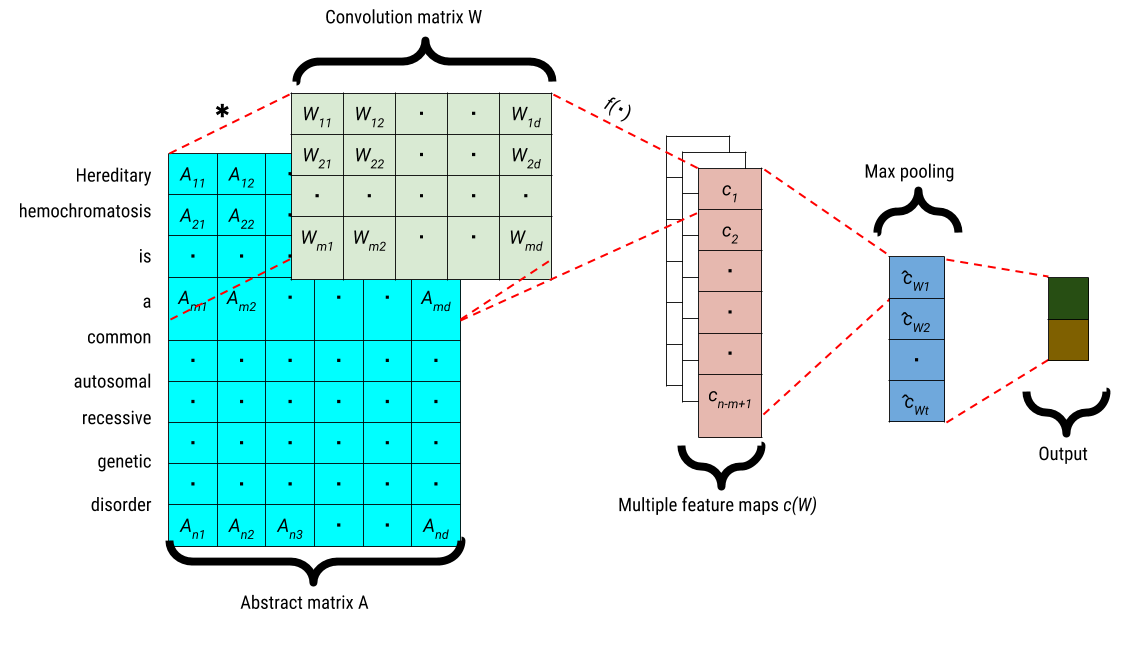
\includegraphics[width=1\textwidth,left]{Figures/cnn-model-example.png}
    \caption{This figure illustrates a CNN with one convolution layer that is precisely used in the experimental setup in this thesis in the context of biomedical abstracts.}
    \label{fig:Cnn_one_layer}
\end{figure}
The basic component of the model is the word vector $\mathbf{x} \in \mathbb{R}^d$, where $d$ is the dimension of the word vectors. An abstract is represented as a matrix $A \in \mathbb{R}^{n \times d}$, where $n$ is the number of words in it. As mentioned earlier in the section~\ref{section:architecture}, each row corresponds to the word vector for the corresponding token or word. For the sake of brevity, we assume that the ground truth (label) for the abstract is $y \in \mathbb{R}^2$ such that $y_2 = 1$ and $y_1 = 0$ ($y_2 = 0$ and $y_1 = 1$) when we are training on a positive (negative) instance. This precisely aligns with the Figure~\ref{fig:Cnn_one_layer} with two output nodes of the final layer for the two classes (positive or negative) for each binary classifier. In this project we perform classification for 48 classes. 
%\todo{mention the number of classes for which the problem is solved !! was it 26 ?}.

We define a kernel $\mathbf{W} \in \mathbb{R}^{m \times d}$, where $m$ is the length of the sliding window. The two-dimensional convolution operation $\mathbf{*}$ can now be defined as follows,

\begin{center}
\[\mathbf{W} * A_{j:j+m-1} = \sum_{i=j}^{j+m-1} \sum_{k=0}^{d-1} \mathbf{W}_{i,k} A_{i,k}.
\]
\end{center}

Next, by using a non-linear function $f(\cdot)$, we map a window of length $m$ to a real number $c_j \in \mathbb{R}$ as 

\[c_j = f(\mathbf{W} * A_{i, j:j+m-1} + b),
\]
 
 where $b \in \mathbb{R}$ is the bias. In this thesis, $f(\cdot)$ is a Rectified Linear Unit (ReLU)~\cite{glorot2011deep, nair2010rectified}. We get the following feature map after convolving over the whole abstract,

 \[\mathbf{c(W)} = [c_1, \ldots, c_{n-m+1}].\]

 Further, to overcome the problem of abstracts of varying lengths, we perform the statistical operation of max-pooling~\cite{zhou1988image} (see also Figure~\ref{fig:maxpool})

 \[\widehat{c_{\mathbf{W}}} = \max_{i} \mathbf{c(W)}_i,\]

 that yields a feature $\widehat{c_{\mathbf{W}}}$ associated to the feature map generated by $\mathbf{W}$. Suppose that we want to learn $t$ kernels $\mathbf{W}^1, \ldots, \mathbf{W}^t$, to obtain multiple features maps. This leads to $t$ single max-pooled features which can be represented as follows,

 \[ \mathbf{\widehat{c_{\mathcal{W}}}} = [\mathbf{\widehat{c_{\mathbf{W}^1}}}, \ldots, \mathbf{\widehat{c_{\mathbf{W}^t}}}],
 \]

 where $\mathcal{W} = \{\mathbf{W}^1, \ldots, \mathbf{W}^t\}$. After this, finally we add a softmax layer. The parameters of the softmax layer $\mathbf{V} \in \mathbb{R}^2 \times t$ and $b^{V} \in \mathbb{R}^2$ with weighted inputs 

 \[y_j = \mathbf{V}_j \mathbf{\widehat{c_{\mathcal{W}}}} + b^{V}_j\]

and output label probability estimates as

\[P(y_j = 1 | A, \mathcal{W}, b, \mathbf{V}, b^{V}) = \frac{e^{y_j}}{\sum_i e^{y_i}},\]

where $\mathbf{V}_j$ $b^{V}_j$ are the $j^{th}$ row and $j^{th}$ element of $\mathbf{V}$ and $b^{V}$ respectively. $y_j$ is the $j^{th}$ label for the abstract corresponding to matrix $A$. 

If $\mathcal{A}$ is the set of training abstract matrices, then in order to learn each binary classifier, we minimize the following loss/objective function

\[- \sum_{A \in \mathcal{A}} \log(P(y_j^A = 1 | A, \mathcal{W}, b, \mathbf{V}, b^{V})),\]

where $j=1$ or $j=2$ depending upon the positive or negative training instance and $y^A$ is the ground truth label for the abstract represented by $A$. The parameters of CNN, that is $(\mathcal{W}, b, \mathbf{V}, b^{V})$ that minimize the loss function are modified by employing the back propagation algorithm with stochastic gradient descent approach. 

As a regularization term so that the model doesn't overfit, we use dropout~\cite{srivastava2014dropout}. More specifically, instead of feeding $y_j$ to the softmax function during training, we actually feed 

\[ \widehat{y_{j}} = \mathbf{V}_j( \mathbf{\widehat{c_{\mathcal{W}}}} \circ \mathbf{s}) + b^{V}_j,
\]
 
where $\circ$ refers to hadamard product (element-wise multiplication) and $\mathbf{s} \in \{0,1\}^t$ is generated with each element $s_i$ drawn from the Bernoulli distribution with parameter $p$ set to $0.2$. In layman terms, this means that the gradients are backpropagated only through those neurons where $s_i = 1$. 

% Note that, while testing the model, we downscale the weights $\mathbf{V}$ such that 

% \[y_j = p\mathbf{V}_j \mathbf{\widehat{c_{\mathcal{W}}}} + b^{V}_j.\]

% This operation is essential because during training, only $80\%$ of the edges are active, that is obviously not true when we test the model. 


\subsubsection{RNN}
Recurrent neural networks~\cite{rumelhart1988learning} are used for processing sequential data. Since language is sequential in nature because when we deal with natural language there is context required for predicting what comes next. RNNs are widely used in natural language models as it used to process sequential data.
As a human being, every time when we try to solve something we don't reboot the brain, instead we remember things and try to build on from that. The traditional neural networks cannot have persistence they always re-learn for scratch unlike human brain, for example if we want to predict what word would come next in the sentence or when we want to do a prediction of the next term in the sequence. In such cases we need the information of what happened previously stored in the network, the RNNs are able to do such computations because they have loops in the network as can be seen in the Figure~\ref{fig:rnnarch}~\cite{chung2015recurrent}. They try to keep track of the information that was learnt previously. 
%Whereas when we deal with natural language there is context required for predicting what comes next, sometimes there is a difference between that there is a big difference between the relevant information and the point where it is needed. 
RNNs do not always perform best when handling ``long term dependencies''~\cite{bengio1994learning}. To overcome this problem, Long Short Term Memory networks (LSTMs) were introduced by~\cite{hochreiter1997long} that are a special kind RNNs which can handle learning the long term dependencies. 

\paragraph{RNN Model Description}
Figure~\ref{fig:rnnarch} introduces the RNN architecture where the input $x_t$ is fed is a hidden layer at time step $t$. 
\begin{figure}
    \centering
    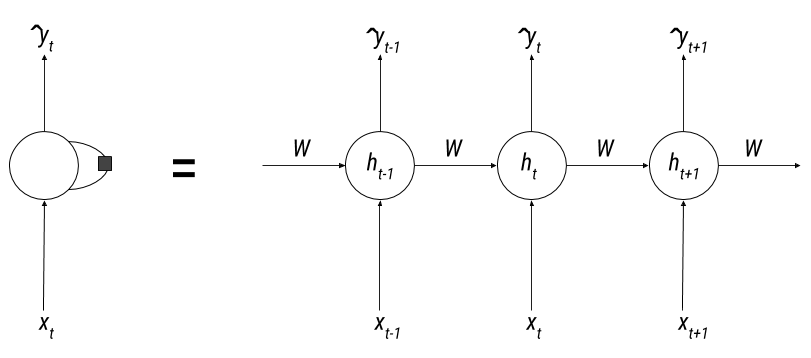
\includegraphics[scale=0.5]{Figures/rnn_figure_1.png}
    \caption{Recurrent Neural Network}
    \label{fig:rnnarch}
\end{figure}
Here, each layer consists of neurons, where each neuron performs a linear matrix operation on its corresponding input which is followed by a non-linear operation. At each time step, the output of the previous step along with the next word vector in the abstract are inputs to the hidden layer that yields $\widehat{y}$ as output and features $h_t$. The inputs and outputs to each neuron in the RNN can be described as follows,

\begin{equation}
\begin{aligned}
	h_t = W f(h_{t-1}) + W^{(hx)}x_t
\end{aligned}
\end{equation}

\begin{equation}
\begin{aligned}
	\widehat{y} = W^{(S)}f(h_{t})
\end{aligned}
\end{equation}

Next, we mention the details associated with each parameter in the network:

\begin{itemize}
	\item Suppose the abstract is of $n$ words in total. Then $x_1, \ldots, x_n$ is the word vectors corresponding to the words of the abstract.

	\item $h_t = \sigma(W^{hh}h_{t-1} + W^{hx}x_t)$ corresponds to the hidden layer features at a particular time step $t$. Here $x_t \in \mathbb{R}^d$ is the input word vector at time step $t$. $W^{hx} \in \mathbb{R}^{D_h \times d}$ and $W^{hh} \in \mathbb{R}^{D_h \times D_h}$ are the weight matrices used to condition input word vector $x_t$ and output of previous time step $h_{t-1}$ respectively.

	\item $\widehat{y}_t = \text{softmax}(W^{(S)} h_t)$ corresponds to the output probability estimates over the vocabulary at each time step $t$. $W^{(S)} \in \mathbb{R}^{|V| \times D_h}$ and $\widehat{y} \in \mathbb{R}^{|V|}$ where $|V|$ is vocabulary.


\end{itemize}

The RNNs are trained using an extension of back propagation algorithm known as back propagation through time (BPPT) algorithm. More specifically, it begins by unfolding the RNN in time: (i) each timestep has one input, one copy of the network (every copy of the network shares the same parameters), and one output, (ii) errors are calculated and accumulated for each timestep, and (iii) the network is rolled back up and the weights are updated.  Then the back propagation algorithm is applied traditionally. The main disadvantage of RNNs is that they can not capture long-term dependencies due to vanishing/exploding gradients during backpropagation. More specifically, if the weights of the word embedding matrix which is input to the RNN are small, it can lead to a vanishing gradients where the gradient signal is so weak that the learning is slow or stops altogether. Conversely, if the weights are large, it can lead to very strong gradient signal that causes the learning to diverge, that is, exploding gradients.

To overcome the problem of long-term dependencies, LSTM was developed, that is, to gain more persistent memory. The mathematical formulation of the LSTM unit is described below,

\begin{equation}
\begin{aligned}
	i^{(t)} = \sigma(W^{(i)}x_t + U^{(i)}h_{t-1}) && \text{(Input \ Gate)} \\
	f^{(t)} = \sigma(W^{(f)}x_t + U^{(f)}h_{t-1}) && \text{(Forget \ Gate)} \\
	o_t = \sigma(W^{(o)}x_t + U^{(o)}h_{t-1}) && \text{(Output \ Gate)} \\
	\widetilde{c}^{(t)} = \text{tanh}(W^{(c)}x_t + U^{(c)}h_{t-1}) && \text{(New \ Memory \ cell)} \\
	c^{(t)} = f^{(t)} \circ \widetilde{c}^{(t-1)} + i^{(t)} \circ \widetilde{c}^{(t)} && \text{(Final \ memory \ cell)} \\
	h^{(t)} = o_t \circ \tanh(c^{(t)})
\end{aligned}
\end{equation}


%\todo{Draw Figure LSTM unit explaining gates}
\begin{figure}[!htb]
    \centering
    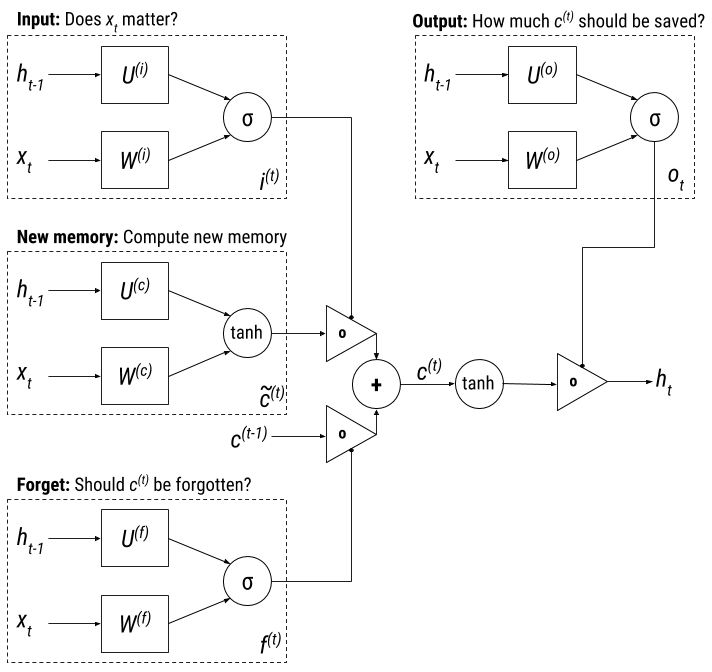
\includegraphics[scale=0.55]{Figures/lstm-unit.png}
    \caption{The detailed internals of a LSTM unit}
    \label{fig:lstmunit}
\end{figure}

Finally, we explain the structure and the intuition behind LSTM units below:

\begin{itemize}
	\item \textbf{New memory generation: }It is the consolidation of a new input word vector $x_t$ with the past hidden state $h_{t-1}$. From the model point of view, this gate cooks the recipe of summarizing the new input in the light of contextual past.

	\item \textbf{Input Gate: }The new memory cell generates new memory blindly without even bothering whether the new input is important or not -- the objective of the input gate is to determine the importance to the new input by using it and the past hidden state. Hence, it is used to gate the new memory and produces $i^{(t)}$ which indicates information.

	\item \textbf{Forget Gate: }The forget gate is analogous to input gate in the sense that it makes an assessment on the usefulness of the past memory cell that is used for the computation of current memory cell. Thus, it looks at the input and the past hidden state and produces $f^{(t)}$.

	\item \textbf{Final memory generation: }Both the input gate and the forget gate act as an advisory to final memory cell, that is, whether to forget past memory or gate new memory respectively. The final memory cell then sums these results to produce the final memory $c^{(t)}$.

	\item \textbf{Output Gate: } Its objective to the separate final memory $c^{(t)}$ from the hidden state. $c^{(t)}$ might not necessarily contain only relevant information all the time that is required to be saved by the hidden state. Moreover, as hidden states are used in every gate of an LSTM unit, the output gate makes an assessment regarding the importance of the information to be stored in the hidden state $h_t$. This produces $o_t$ and this is to gate the point-wise $tanh$ of the memory.
\end{itemize}

The bi-directional version of RNN or LSTM, at each time-step $t$, maintains two hidden layers, one for left-to-right propagation and another for right-to-left propagation. Clearly, this consumes two times as much memory as RNNs. The final output $\widehat{y_t}$ is obtained by combining the scores computed by both the hidden states.



%\input{chapters/data.tex}
\chapter{Results and Discussion}\label{chap: results}

We start by presenting an elementary approach to this research problem. Then we move on to the comparison of results (judging mainly by the accuracy). The results are presented using the neural network model and it is compared with baseline methods. The comparison is divided into two parts (i) first, predicting the disease terms and (ii) second, predicting the super class of the disease terms.

The dataset was tested with three types of problem transformations (refer Section~\ref{MLtranform}): (i) Binary Relevance, (ii) Label Powerset and (iii) Classifier Chains. The problem transformations were used from scikit-multilearn that is a library specific to multi-label classification built on top of the well-known scikit-learn.~\cite{2017arXiv171100046S}. The classifiers that were tested using these transformations were 
\begin{itemize}
    \item Multi-layer Perceptron classifier (MLP classifier) 
    \item Multi-label k Nearest Neighbour (MLkNN) 
    \item Random Forest Classifier 
    \item Decision Trees Classifier 
\end{itemize}
For each combination the evaluation metrics used were: accuracy, hamming loss, weighted F1 score and weighted precision score. The classifiers used and the metrics were calculated using scikit-learn~\cite{scikit-learn}. 

For the neural network approach we utilized the pretrained word embeddings - GloVe: Global Vectors for Word Representation~\cite{pennington2014glove} of length 300. For data preprocessing we used tokenizer API from Keras~\cite{chollet2015keras}. The CNN and BiLSTM architectures were used from PyTorch\footnote{\url{https://pytorch.org/}}.
For validating the results using the Neural Networks we split the data into training and validation sets. The training set is 80\% of the whole data and the validation set is the rest 20\%. A similar train-test split was done for the baseline mu;ti-label classification 80\%-20\%. The dropout rate has been kept $0.2$ in all the neural network models. 

\section{An elementary approach}
In prediction of metadata, specifically diseases - an elementary approach would be to use a vocabulary of disease names, and perform a basic search in the documents. If we have a match it can be said that a particular publication talks about `xyz' disease. This would be a direct and trivial way to approach this problem. 

In this case, since the dataset majorly uses the MeSH ontology, so all the values of disease names is downloaded\footnote{\url{http://bioportal.bioontology.org/ontologies/MESH/?p=classes&conceptid=root}}. After that, a direct matching is done using Flashtext~\cite{2017arXiv171100046S}. Firstly the downloaded diseases from the MeSH contains a lot of secondary information which is not essential, therefore columns with disease names are selected. This also includes the synonyms so that the matching is not biased for terms like `heart disease' and `cardiovascular disease'. Even after including the synonyms we could find only $44$ unique terms in the text, which is $\approx$2\% of the diseases identified disease terms.



\section{Predicting Disease Terms}
For prediction of disease terms, the unique ID (explained in Section~\ref{section:data}) were used as labels after preprocessing - removing duplicates and characters if present. 

\subsection{Baseline Multi-label Classification}
For baseline multi-label classification two type of feature extraction techniques were used: (i) TF-IDF and (ii) Bag of words representation (BoW). The results for these two techniques are presented in Tables~\ref{tab:resultdiseasetfidf} and~\ref{tab:resultdiseasecount}. For both the techniques the maximum feature length is kept 200. It can be seen that the MLP Classifier performs the best in both the techniques of feature extraction. 

There is a difference in the performance if we compare the different feature extraction methods, the TF-IDF technique performs better. The TF-IDF normalizes the outputs which is why this technique is known to perform better when comes to the feature selection, it can be observed from the results as well. 
Since dataset has a large number of diseases - $588$, and a limited number of abstracts, the accuracy of predictions is not very high. The highest accuracy that we get here is $\approx 19\%$. 

\begin{table}[!htb]
    \centering
    \resizebox{\textwidth}{!}{%
\begin{tabular}{|c|l|l|l|l|l|l|l|l|l|l|l|l|l|}
\hline
\multicolumn{1}{|l|}{\multirow{2}{*}{}}                               & \multicolumn{3}{c|}{Random forest}                                          & \multicolumn{3}{c|}{Decision Tree}                                          & \multicolumn{3}{c|}{MLPClassifier}                                          & \multicolumn{4}{c|}{MLkNN}                                                                                   \\ \cline{2-14} 
\multicolumn{1}{|l|}{}                                                & \multicolumn{1}{c|}{BR} & \multicolumn{1}{c|}{LP} & \multicolumn{1}{c|}{CC} & \multicolumn{1}{c|}{BR} & \multicolumn{1}{c|}{LP} & \multicolumn{1}{c|}{CC} & \multicolumn{1}{c|}{BR} & \multicolumn{1}{c|}{LP} & \multicolumn{1}{c|}{CC} & \multicolumn{1}{c|}{k=20} & \multicolumn{1}{c|}{k=30} & \multicolumn{1}{c|}{k=10} & \multicolumn{1}{c|}{k=5} \\ \hline
Accuracy                                                              & \textbf{0.101}          & 0.075                   & 0.088                   & 0.044                   & \textbf{0.107}          & 0.082                   & 0.170                   & \textbf{0.189}          & 0.164                   & 0.164                     & 0.138                     & \textbf{0.176}            & \textbf{0.176}           \\ \hline
hamming loss                                                          & 0.004                   & 0.007                   & 0.004                   & 0.007                   & 0.007                   & 0.007                   & 0.004                   & 0.005                   & 0.004                   & 0.004                     & 0.004                     & 0.004                     & 0.004                    \\ \hline
\begin{tabular}[c]{@{}c@{}}F1 score \\ (weighted)\end{tabular}        & 0.125                   & 0.191                   & 0.117                   & 0.259                   & 0.208                   & 0.250                   & 0.207                   & 0.233                   & 0.203                   & 0.194                     & 0.184                     & 0.238                     & 0.232                    \\ \hline
\begin{tabular}[c]{@{}c@{}}precision score \\ (weighted)\end{tabular} & 0.226                   & 0.197                   & 0.188                   & 0.264                   & 0.235                   & 0.250                   & 0.226                   & 0.250                   & 0.234                   & 0.218                     & 0.231                     & 0.258                     & 0.263                    \\ \hline
\end{tabular}%
}
    \caption{Results for Disease terms using TF-IDF feature selection}
    \label{tab:resultdiseasetfidf}
\end{table}

\begin{table}[!htb]
    \centering
    \resizebox{\textwidth}{!}{%
\begin{tabular}{|c|l|l|l|l|l|l|l|l|l|l|l|l|l|}
\hline
\multicolumn{1}{|l|}{\multirow{2}{*}{}} & \multicolumn{3}{c|}{Random forest} & \multicolumn{3}{c|}{Decision Tree} & \multicolumn{3}{c|}{MLPClassifier} & \multicolumn{4}{c|}{MLkNN} \\ \cline{2-14} 
\multicolumn{1}{|l|}{} & \multicolumn{1}{c|}{BR} & \multicolumn{1}{c|}{LP} & \multicolumn{1}{c|}{CC} & \multicolumn{1}{c|}{BR} & \multicolumn{1}{c|}{LP} & \multicolumn{1}{c|}{CC} & \multicolumn{1}{c|}{BR} & \multicolumn{1}{c|}{LP} & \multicolumn{1}{c|}{CC} & \multicolumn{1}{c|}{k=20} & \multicolumn{1}{c|}{k=30} & \multicolumn{1}{c|}{k=10} & \multicolumn{1}{c|}{k=5} \\ \hline
Accuracy & 0.088 & \textbf{0.126} & 0.088 & 0.082 & 0.094 & \textbf{0.113} & 0.132 & \textbf{0.157} & 0.126 & 0.088 & 0.088 & \textbf{0.107} & 0.082 \\ \hline
hamming loss & 0.004 & 0.006 & 0.004 & 0.008 & 0.008 & 0.008 & 0.004 & 0.005 & 0.004 & 0.004 & 0.004 & 0.004 & 0.005 \\ \hline
\begin{tabular}[c]{@{}c@{}}F1 score \\ (weighted)\end{tabular} & 0.106 & 0.160 & 0.090 & 0.256 & 0.191 & 0.257 & 0.175 & 0.217 & 0.171 & 0.098 & 0.091 & 0.128 & 0.163 \\ \hline
\begin{tabular}[c]{@{}c@{}}precision score \\ (weighted)\end{tabular} & 0.158 & 0.178 & 0.152 & 0.250 & 0.216 & 0.262 & 0.217 & 0.241 & 0.216 & 0.166 & 0.167 & 0.172 & 0.199 \\ \hline
\end{tabular}%
}
    \caption{Results for Disease terms using Bag of words feature selection}
    \label{tab:resultdiseasecount}
\end{table}

\subsection{Neural Network Method}
For the neural network method. Two models were trained - (i) BiLSTM and (ii) CNN. The embedding dimension in both cases is 300, where the input sequences are kept as 200 for which the results are discussed. The models are also retrained for a sequence length of 150 and 250 to check whether the accuracy increases or decreases. The models are trained using the Adam optimizer~\cite{kingma2014adam}. 

The results of models are presented in Table~\ref{tab:DLdiseases}. The number of epochs are kept high because of a large number of labels. Here it can be seen that the CNN outperforms all the baseline methods and the BiLSTM. Whereas the BiLSTM has a lesser accuracy than highest baseline MLP classifier. One explanation would be that since the RNN treats the input as a sequence, and its a very long sequence, as it goes ahead working on word after word, it forgets what happened in the words before. Even though we're using a bidirectional RNN, maybe the left to right forgets what happened at the start, say by the time it reaches mid sequence, and the right to left forgets what it saw in the first (rightmost) terms by the time it reaches mid sequence too. 

Whereas in CNNs, the convolution kernels are time invariant so they cannot distinguish between different parts of the sequence. As a disadvantage, they cannot easily do inferences which require using context, and need to treat the input as a sequence. However in this case, it might not be needed. Abstracts may somewhere mention a particular disease keyword  which is enough on its own to detect which class it belongs to (and this detection requires no sequential treatment of input, which is similar to `find a word').

\begin{table}[!htb]
\centering
\begin{tabular}{|l|l|l|l|}
\hline
\multicolumn{1}{|c|}{} & \multicolumn{1}{c|}{\textbf{Epochs}} & \multicolumn{1}{c|}{\textbf{\begin{tabular}[c]{@{}c@{}}Validation \\ Accuracy\end{tabular}}} & \multicolumn{1}{c|}{\textbf{\begin{tabular}[c]{@{}c@{}}Sequence\\  Length\end{tabular}}} \\ \hline
\textbf{BiLSTM} & 200 & \textit{\textbf{0.177}} & 200 \\ \hline
 & 200 & 0.168 & 150 \\ \hline
 & 200 & 0.099 & 250 \\ \hline
\textbf{CNN} & 180 & 0.31 & 200 \\ \hline
 & 180 & 0.283 & 150 \\ \hline
 & 180 & \textit{\textbf{0.335}} & 250 \\ \hline
\end{tabular}
\caption{Results for deep neural networks for predicting disease names}
\label{tab:DLdiseases}
\end{table}

\section{Predicting Super Class}
In this experiment we use the MeSH tree structure\footnote{\url{https://meshb.nlm.nih.gov/treeView}} to map the annotated disease names to their super classes shown in Figure~\ref{fig:meshsuperclass}. 
\begin{figure}[!htb]
    \centering
    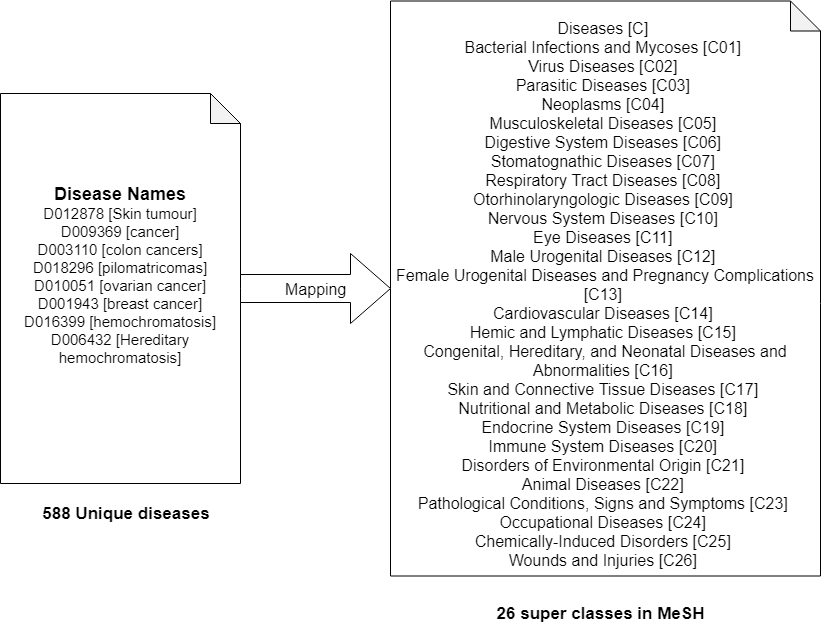
\includegraphics[scale=0.45]{Figures/NN_prediction.png}
    \caption{Mapping super classes in MeSH}
    \label{fig:meshsuperclass}
\end{figure}
To do so we use the unique ID of the disease terms as explained in Section~\ref{section:data} to do a SPARQL query to map these terms (refer Listing~\ref{superclassquery}). The motivation behind this experiment setup is to reduce the number of labels that the method had to predict. This is done for each abstract, then these new super classes are used as target labels. 

A discrepancy when mapping the super classes is that when queried for all the diseases, we got 48 super classes rather than 26. The classes ``Disorders of Environmental Origin [C21], Animal Diseases [C22]'' are not identified as super classes for any diseases. Furthermore, there are 24 additional classes are identified:
\begin{spverbatim}
`Physical Phenomena', `Genetic Phenomena', `Population Characteristics', `Nonsyndromic sensorineural hearing loss', `Diagnosis', `Physiological Phenomena', `Psychological Phenomena', `Cell Physiological Phenomena', `Investigative Techniques', `Biological Phenomena', `Behavior and Behavior Mechanisms', `Immune System Phenomena', `Reproductive and Urinary Physiological Phenomena', `Fluids and Secretions', `Cells', `Health Occupations', `Environment and Public Health', `Tissues', `Mental Disorders', `Behavioral Disciplines and Activities', `Musculoskeletal and Neural Physiological Phenomena', `Therapeutics', `Health Care Quality, Access, and Evaluation', `Natural Science Disciplines'. 
\end{spverbatim}
This could be due to the fact that disease names is not linked to super class as the abstract text could contain another synonym word. 
For example: the term `Genetic Phenomena (ID: [G05])' a super class itself as can be seen in \url{https://meshb.nlm.nih.gov/treeView}, it comes under the parent class of ``Phenomena and Processes [G]''. 
%For example: `Nonsyndromic sensorineural hearing loss'  this was not annotated to ``preferred label", which is why query couldn't map to the DOI of super class.

\begin{lstlisting}[caption = SPARQL query to map disease names to their respective super classes, label = superclassquery]
PREFIX rdf: <http://www.w3.org/1999/02/22-rdf-syntax-ns#>
PREFIX rdfs: <http://www.w3.org/2000/01/rdf-schema#>
PREFIX xsd: <http://www.w3.org/2001/XMLSchema#>
PREFIX owl: <http://www.w3.org/2002/07/owl#>
PREFIX meshv: <http://id.nlm.nih.gov/mesh/vocab#>
PREFIX mesh: <http://id.nlm.nih.gov/mesh/>
PREFIX mesh2015: <http://id.nlm.nih.gov/mesh/2015/>
PREFIX mesh2016: <http://id.nlm.nih.gov/mesh/2016/>
PREFIX mesh2017: <http://id.nlm.nih.gov/mesh/2017/>
PREFIX mesh2018: <http://id.nlm.nih.gov/mesh/2018/>
PREFIX mesh2019: <http://id.nlm.nih.gov/mesh/2019/>
SELECT DISTINCT ?p ?label ?uri 
    WHERE { mesh:D012878 meshv:broaderDescriptor* ?uri .
            ?uri rdfs:label ?p.
            FILTER NOT EXISTS{
            ?uri meshv:broaderDescriptor ?x
        }
    }
\end{lstlisting}

%write about the data discrepancy. 

\subsection{Baseline Multi-label Classification}
The results for the baselines are present in Table~\ref{tab:resulttfidf}, here the features were extracted using TF-IDF. Another set of features were extracted using bag of word representation, the results are shown in the Table~\ref{tab:resultsBOW}. The maximum number of features for both the feature extraction techniques is kept to be 200. 
The Label Powerset transformation gives better performance for all three baseline classifiers. Overall, the Random forest classifier has the highest accuracy with problem transformation of Label Powerset. 

In this setup the feature extraction using bag of words technique has a better performance when compared to TF-IDF. An explanation behind this would be that in a random forest classification method when given a set of features and labels it creates random subsets of features and building decision trees with the help of these subsets after which it makes predictions. 

%For MLP classifier the obtained are shown in the Table~\ref{table:MLP}. It can be seen that the classifier performs very poorly and the accuracy is 0 for the transformations of Binary Relevance and classifier chains. 

\begin{table}[!htb]
\centering
% \hskip-2.2cm
\resizebox{\textwidth}{!}{\begin{tabular}{|c|l|l|l|l|l|l|l|l|l|l|l|l|l|}
\hline
\multirow{2}{*}{} & \multicolumn{3}{c|}{Random forest} & \multicolumn{3}{c|}{Decision Tree} & \multicolumn{3}{c|}{MLPClassifier} & \multicolumn{4}{c|}{MLkNN} \\ \cline{2-14} 
 & \multicolumn{1}{c|}{BR} & \multicolumn{1}{c|}{LP} & \multicolumn{1}{c|}{CC} & \multicolumn{1}{c|}{BR} & \multicolumn{1}{c|}{LP} & \multicolumn{1}{c|}{CC} & \multicolumn{1}{c|}{BR} & \multicolumn{1}{c|}{LP} & \multicolumn{1}{c|}{CC} & \multicolumn{1}{c|}{k=20} & \multicolumn{1}{c|}{k=30} & \multicolumn{1}{c|}{k=10} & \multicolumn{1}{c|}{k=5} \\ \hline
Accuracy & 0.181 & \textbf{0.348} & 0.174 & 0.148 & \textbf{0.271} & 0.135 & 0.232 & \textbf{0.348} & 0.335 & 0.303 & 0.284 & \textbf{0.316} & 0.297 \\ \hline
\begin{tabular}[c]{@{}c@{}}hamming \\ loss\end{tabular} & 0.050 & 0.058 & 0.052 & 0.059 & 0.068 & 0.063 & 0.050 & 0.044 & 0.049 & 0.045 & 0.044 & 0.044 & 0.045 \\ \hline
\begin{tabular}[c]{@{}c@{}}F1 score\\ (weighted)\end{tabular} & 0.605 & 0.642 & 0.572 & 0.676 & 0.632 & 0.662 & 0.669 & 0.712 & 0.668 & 0.670 & 0.669 & 0.681 & 0.683 \\ \hline
\begin{tabular}[c]{@{}c@{}}precision score\\ (weighted)\end{tabular} & 0.804 & 0.711 & 0.823 & 0.686 & 0.632 & 0.681 & 0.712 & 0.799 & 0.734 & 0.788 & 0.802 & 0.783 & 0.821 \\ \hline
\end{tabular}}
    \caption{Results of predicting super class using TF-IDF feature selection}
    \label{tab:resulttfidf}
\end{table}

\begin{table}[!htb]
    \centering
    \resizebox{\textwidth}{!}{%
\begin{tabular}{|c|l|l|l|l|l|l|l|l|l|l|l|l|l|}
\hline
\multicolumn{1}{|l|}{\multirow{2}{*}{}} & \multicolumn{3}{l|}{Random forest} & \multicolumn{3}{l|}{Decision Tree} & \multicolumn{3}{l|}{MLPClassifier} & \multicolumn{4}{c|}{MLkNN} \\ \cline{2-14} 
\multicolumn{1}{|l|}{} & \multicolumn{1}{c|}{BR} & \multicolumn{1}{c|}{LP} & \multicolumn{1}{c|}{CC} & \multicolumn{1}{c|}{BR} & \multicolumn{1}{c|}{LP} & \multicolumn{1}{c|}{CC} & \multicolumn{1}{c|}{BR} & \multicolumn{1}{c|}{LP} & \multicolumn{1}{c|}{CC} & \multicolumn{1}{c|}{k=20} & \multicolumn{1}{c|}{k=30} & \multicolumn{1}{c|}{k=10} & \multicolumn{1}{c|}{k=5} \\ \hline
Accuracy & 0.168 & \textbf{0.368} & 0.200 & 0.116 & \textbf{0.329} & 0.168 & 0.258 & \textbf{0.342} & 0.303 & \textbf{0.148} & 0.097 & 0.142 & 0.142 \\ \hline
Hamming Loss & 0.049 & 0.053 & 0.054 & 0.065 & 0.060 & 0.070 & 0.047 & 0.049 & 0.047 & 0.059 & 0.061 & 0.062 & 0.063 \\ \hline
\begin{tabular}[c]{@{}c@{}}F1 score\\ (weighted)\end{tabular} & 0.605 & 0.649 & 0.554 & 0.641 & 0.657 & 0.630 & 0.668 & 0.672 & 0.674 & 0.520 & 0.510 & 0.521 & 0.531 \\ \hline
\begin{tabular}[c]{@{}c@{}}Precision score\\ (weighted)\end{tabular} & 0.816 & 0.717 & 0.782 & 0.661 & 0.702 & 0.637 & 0.766 & 0.758 & 0.764 & 0.737 & 0.681 & 0.692 & 0.660 \\ \hline
\end{tabular}%
}
    \caption{Results of predicting super class using Bag of words feature selection}
    \label{tab:resultsBOW}
\end{table}

\subsection{Neural Network Method}
For the neural network method.  Two models were trained - (i) BiLSTM and (ii)
CNN. The dimension of the embedding matrix in both cases is 300, where the input sequences of the abstract
are kept as 200 for which the results are discussed. The models are also retrained
for a sequence length of 150 and 250 to check whether the accuracy increases or
decreases. The models are trained using the Adam optimizer~\cite{kingma2014adam}. The results are shown in the Table~\ref{tab:DLsuperclass}. The number of epochs is kept to 65 as the number of labels is not high as in the previous setup. 

Here both the BiLSTM and CNN outperform all the baseline classifiers. Overall, the CNN has highest performance accuracy with the sequence length of 200. Another interesting observation is that when the sequence length is increased to 250 the accuracy of the BiLSTM increases, whereas one would think it should decrease because LSTMs tend to forget what happened previously or ahead when the sequence length is increased. One explanation behind this could be that the disease words occur towards the end in the abstract. 

\begin{table}[!htb]
    \centering
    \begin{tabular}{|l|c|c|c|}
\hline
\multicolumn{1}{|c|}{} & \textbf{Epochs} & \textbf{\begin{tabular}[c]{@{}c@{}}Validation \\ Accuracy\end{tabular}} & \textbf{\begin{tabular}[c]{@{}c@{}}Sequence\\  Length\end{tabular}} \\ \hline
\textbf{BiLSTM} & 65 & 0.623 & 200 \\ \hline
 & 65 & 0.628 & 150 \\ \hline
 & 65 & \textit{\textbf{0.697}} & 250 \\ \hline
\textbf{CNN} & 60 & \textit{\textbf{0.837}} & 200 \\ \hline
 & 60 & 0.76 & 150 \\ \hline
 & 60 & 0.803 & 250 \\ \hline
\end{tabular}
    \caption{Results for deep neural networks for predicting super class}
    \label{tab:DLsuperclass}
\end{table}


\section{Discussion}
In this section we mainly discuss the results that we get using the neural network method, specifically for the sequence length of 200. The reason why we keep this as a gold standard input length is because it is closest to the mean length of the number of words in all the abstracts (refer Section~\ref{section:data}). For this we pick three abstracts that are present common in the validation set of both the disease name and super class experiment. Note that the text is preprocessed. 

\newenvironment{boxet}
    {\begin{center}
    \begin{tabular}{|p{0.9\textwidth}|}
    \hline\\
    }
    { 
    \\\\\hline
    \end{tabular} 
    \end{center}
    }
    %--------------------------------------------------
\begin{boxet}
Abstract 1: \textsf{promoter luciferase constructs were transiently cotransfected with a wild type vhl wt vhl vector in several cell lines including 293 embryonic kidney and rcc cell lines wt vhl protein inhibited vegf promoter activity in a dose dependent manner up to 5 to 10 fold deletion analysis defined a 144 bp region of the vegf promoter necessary for vhl repression this vhl responsive element is gc rich and specifically binds the transcription factor sp1 in crude nuclear extracts in drosophila cells cotransfected vhl represses sp1 mediated activation but not basal activity of the vegf promoter we next demonstrated in coimmunoprecipitates that vhl and sp1 were part of the same complex and by using a glutathione s transferase vhl fusion protein and purified sp1 that vhl and sp1 directly interact furthermore endogenous vegf mrna levels were suppressed in permanent rcc cell lines expressing wt vhl and nuclear run on studies indicated that vhl regulation of vegf occurs at least partly at the transcriptional level these observations support a new mechanism for vhl mediated transcriptional repression via a direct inhibitory action on sp1 and suggest that loss of sp1 inhibition may be important in the pathogenesis of von hippel lindau disease and rcc.}

Actual labels: 

\emph{Superclass} - [`Congenital, Hereditary, and Neonatal Diseases and Abnormalities', `Nervous System Diseases', `Cardiovascular Diseases', `Male Urogenital Diseases', `Female Urogenital Diseases and Pregnancy Complications', `Skin and Connective Tissue Diseases', `Neoplasms']

\emph{Disease Names} - [`von Hippel-Lindau Disease', `Carcinoma, Renal Cell'].
\end{boxet}
\begin{boxet}
Abstract 2: \textsf{we have analyzed the 27 exons and the promoter region of the rb1 gene in familial or sporadic bilateral retinoblastoma by using single strand conformation polymorphism analysis for improvement over previous studies a new set of primers has been designed which allow for amplification of the coding and splicing sequences only the positioning of the polymerase chain reaction pcr primers was such that the resulting pcr products were of different sizes which enabled us to analyze two different exons simultaneously and still distinguish between the banding profiles for both biplex analysis by using this approach we were able to identify mutation in 22 new patients but the overall efficiency of the procedure when we used a single pass regimen was only 48 the mutations were small insertions and deletions and point mutations in roughly equal proportions}

Actual labels:\emph{Super class} -  [`Congenital, Hereditary, and Neonatal Diseases and Abnormalities', `Neoplasms', `Eye Diseases']

\emph{Disease names} - [`Retinoblastoma']
\end{boxet}
\begin{boxet}
Abstract 3: \textsf{programmed cell death or apoptosis is a physiological process essential to the normal development and homeostatic maintenance of the immune system the fas apo 1 receptor plays a crucial role in the regulation of apoptosis as demonstrated by lymphoproliferation in mrl lpr lpr mice and by the recently described autoimmune lymphoproliferative syndrome alps in humans both of which are due to mutations in the fas gene we describe a novel family with alps in which three affected siblings carry two distinct missense mutations on both the fas gene alleles and show lack of fas induced apoptosis the children share common clinical features including splenomegaly and lymphadenopathy but only one developed severe autoimmune manifestations in all three siblings we demonstrated the presence of anergic cd3 cd4 cd8 double negative dn t cells moreover a chronic lymphocyte activation was found as demonstrated by the presence of high levels of hla dr expression on peripheral cd3 cells and by the presence of high levels of serum activation markers such as soluble interleukin 2 receptor sll 2r and soluble cd30 scd30}

Actual Label: \emph{Super class} - [`Congenital, Hereditary, and Neonatal Diseases and Abnormalities', `Pathological Conditions, Signs and Symptoms', `Immune System Diseases', `Hemic and Lymphatic Diseases']

\emph{Disease Names} - [`Autoimmune Lymphoproliferative Syndrome', `Splenomegaly', `Lymphatic Diseases', `Autoimmune Diseases']

\end{boxet}

\begin{table}[!htb]
    \centering
\begin{tabular}{|l|l|l|}
\hline
\multicolumn{1}{|c|}{} & \multicolumn{2}{c|}{CNN} \\ \hline
\multicolumn{1}{|c|}{} & \multicolumn{1}{c|}{Disease Name} & \multicolumn{1}{c|}{Super Class} \\ \hline
Abstract 1 & [ ] & \begin{tabular}[c]{@{}l@{}}`Cardiovascular Diseases',\\  `Female Urogenital Diseases and Pregnancy Complications', \\  `Nervous System Diseases', `Skin and Connective Tissue Diseases', \\ `Nutritional and Metabolic Diseases', `Neoplasms', \\ `Congenital, Hereditary, and Neonatal Diseases and Abnormalities'\end{tabular} \\ \hline
Abstract 2 & `Retinoblastoma' & \begin{tabular}[c]{@{}l@{}}`Congenital, Hereditary, and Neonatal Diseases and Abnormalities', \\ `Neoplasms', `Eye Diseases\end{tabular} \\ \hline
Abstract 3 & [ ] & `Congenital, Hereditary, and Neonatal Diseases and Abnormalities' \\ \hline
\end{tabular}
    \caption{Prediction by CNN for the three abstracts}
    \label{tab:predictions_cnn}
\end{table}

\begin{table}[!htb]
    \centering
\begin{tabular}{|l|l|l|}
\hline
\multicolumn{1}{|c|}{} & \multicolumn{2}{c|}{BiLSTM} \\ \hline
\multicolumn{1}{|c|}{} & \multicolumn{1}{c|}{Disease Name} & \multicolumn{1}{c|}{Super Class} \\ \hline
Abstract 1 & `Neoplasms' & \begin{tabular}[c]{@{}l@{}}`Cardiovascular Diseases', `Neoplasms', \\ `Skin and Connective Tissue Diseases'\end{tabular} \\ \hline
Abstract 2 & [ ] & \begin{tabular}[c]{@{}l@{}}`Neoplasms', `Digestive System Diseases', \\ `Congenital, Hereditary, and Neonatal Diseases and Abnormalities', \\ `Skin and Connective Tissue Diseases'\end{tabular} \\ \hline
Abstract 3 & [ ] & \begin{tabular}[c]{@{}l@{}}`Immune System Diseases', `Hemic and Lymphatic Diseases', \\ `Congenital, Hereditary, and Neonatal Diseases and Abnormalities', \\ `Cardiovascular Diseases', `Nutritional and Metabolic Diseases'\end{tabular} \\ \hline
\end{tabular}
    \caption{Prediction by BiLSTM for the three abstracts}
    \label{tab:preidictions_lstm}
\end{table}

The predictions of the three abstracts are presented in Tables~\ref{tab:predictions_cnn} and~\ref{tab:preidictions_lstm}. From the predictions it can be seen when we use a large number of labels in most of abstract there is no prediction at all fo both CNN and BiLSTM. For this we need a larger data for the models to train on. If we get a larger annotated set, the model will be able to learn in a much better way as it would have seen a lot of examples for such a large set of labels.  

Whereas when predicting a super class CNN is very accurate as it would have seen enough examples to learn which label would fit where. Similarly, BiLSTM is accurate more than 50\% of times overall even in some cases where CNN isn't, for example in Abstract 3. This could be because in this case the context of the language would be required more rather than in the other cases. 








%%%%%%%%%%%%%%%%%%%%%%%%%%%%%%%%%%%%%%%%%%%%%%%%%%%%%%%%%%%%%%%%%%%%%%%%%%%%%%%%%%%%%%%%%%%%%%%%%%%
%%%%%%%%%%%%%%%%% commented out section - don't read %%%%%%%%%%%%%%%%%%%%%%%%%%%%%%%%%%%%%%%%%%
%%%%%%%%%%%%%%%%%%%%%%%%%%%%%%%%%%%%%%%%%%%%%%%%%%%%%%%%%%%%%%%%%%%%%%%%%%%%%%%%%%%%%%%%%%%%%%%%%%
\iffalse
\begin{table}[!htb]
\begin{tabular}{|l|c|c|c|}
\hline
MLP Classifier           & \multicolumn{1}{l|}{Binary Relevance} & \multicolumn{1}{l|}{Label Powerset} & \multicolumn{1}{l|}{Classifier Chains} \\ \hline
Accuracy                 & 0.232                                 & 0.348                               & 0.335                                  \\ \hline
Hamming Loss             & 0.050                                 & 0.044                               & 0.049                                  \\ \hline
Weighted F1 score        & 0.669                                 & 0.712                               & 0.668                                  \\ \hline
Weighted Precision score & 0.712                                 & 0.799                               & 0.734                                  \\ \hline
\end{tabular}
\caption{Results for MLP classifier}
\label{table:MLP}
\end{table}




\begin{table}[!htb]
    \centering
    \begin{tabular}{|l|c|c|c|}
\hline
Random Forest Classifier & \multicolumn{1}{l|}{Binary Relevance} & \multicolumn{1}{l|}{Label Powerset} & \multicolumn{1}{l|}{Classifier Chains} \\ \hline
Accuracy                 & 0.181                                 & 0.348                               & 0.174                                  \\ \hline
Hamming Loss             & 0.050                                 & 0.058                               & 0.052                                  \\ \hline
Weighted F1 score        & 0.605                                 & 0.642                               & 0.572                                  \\ \hline
Weighted Precision score & 0.804                                 & 0.711                               & 0.823                                  \\ \hline
\end{tabular}
    \caption{Results for Random Forest Classifier}
    \label{tab:randomforest}
\end{table}

\begin{table}[!htb]
    \centering
\begin{tabular}{|l|c|c|c|}
\hline
Decision Tree Classifier    & \multicolumn{1}{l|}{Binary Relevance} & \multicolumn{1}{l|}{Label Powerset} & \multicolumn{1}{l|}{Classifier Chains} \\ \hline
Accuracy                 & 0.148                                 & 0.271                               & 0.135                                  \\ \hline
Hamming Loss             & 0.059                                 & 0.068                               & 0.063                                  \\ \hline
Weighted F1 score        & 0.676                                 & 0.632                               & 0.662                                  \\ \hline
Weighted Precision score & 0.686                                 & 0.632                               & 0.681                                  \\ \hline
\end{tabular}
    \caption{Results for Decision Tree Classifier}
    \label{tab:decisiontree}
\end{table}

\begin{table}[!htb]
    \centering
    \begin{tabular}{|l|c|c|c|l|}
\hline
MLkNN                    & \multicolumn{1}{l|}{k=20} & \multicolumn{1}{l|}{k=30} & \multicolumn{1}{l|}{k=10} & k=5   \\ \hline
Accuracy                 & 0.303                     & 0.284                     & 0.316                     & 0.297 \\ \hline
Hamming Loss             & 0.045                     & 0.044                     & 0.044                     & 0.045 \\ \hline
Weighted F1 score        & 0.670                     & 0.669                     & 0.681                     & 0.683 \\ \hline
Weighted Precision score & 0.788                     & 0.802                     & 0.783                     & 0.821 \\ \hline
\end{tabular}
    \caption{Results for kNN adaptation for Multilabel Classfication}
    \label{tab:MLkNN}
\end{table}
\begin{table}[!htb]
    \centering
    \begin{tabular}{|l|c|c|c|}
\hline
Gradient Boost Classifier & \multicolumn{1}{l|}{Binary Relevance} & \multicolumn{1}{l|}{Label Powerset} & \multicolumn{1}{l|}{Classifier Chains} \\ \hline
Accuracy                   & 0.0                                   & 0.019                               & 0.006                                  \\ \hline
Hamming Loss               & 0.114                                 & 0.133                               & 0.112                                  \\ \hline
Weighted F1 score          & 0.3                                   & 0.349                               & 0.3                                    \\ \hline
Weighted Precision score   & 0.319                                 & 0.354                               & 0.345                                  \\ \hline
\end{tabular}
    \caption{Results for Gradient Boost Classifier}
    \label{tab:gradientboost}
\end{table}

\begin{table}[!htb]
    \centering
    \begin{tabular}{|l|c|c|c|}
\hline
Linear SVC Classifier    & \multicolumn{1}{l|}{Binary Relevance} & \multicolumn{1}{l|}{Label Powerset} & \multicolumn{1}{l|}{Classifier Chains} \\ \hline
Accuracy                 & 0.0                                   & 0.0452                              & 0.0                                    \\ \hline
Hamming Loss             & 0.152                                 & 0.108                               & 0.147                                  \\ \hline
Weighted F1 score        & 0.375                                 & 0.321                               & 0.378                                  \\ \hline
Weighted Precision score & 0.369                                 & 0.335                               & 0.365                                  \\ \hline
\end{tabular}
    \caption{Results for Linear SVC Classifier}
    \label{tab:linearsvc}
\end{table}


\section{Baseline Method}
In the basic method which involves prediction of metadata, specifically diseases. A baseline method would be to use a vocabulary of disease names, and perform a basic search in the documents. If we have a match it can be said that a particular publication talks about `xyz' disease. This would be a direct and trivial way to approach this problem. 

In this case, since the dataset uses majorly  the MeSH ontology, so all the values of disease names is downloaded\footnote{\url{http://bioportal.bioontology.org/ontologies/MESH/?p=classes&conceptid=root}}. After that, a direct matching is done using Flashtext~\cite{2017arXiv171100046S}. Firstly the downloaded diseases from the MeSH contains a lot of secondary information which is not essential, therefore columns with disease names are selected. This also includes the synonyms so that the matching is not biased for terms like `heart disease' and `cardiovascular disease'. Even after including the synonyms we could find only $44$ unique terms in the text, which is $\approx$2\% of the diseases identified disease terms. 
%write the results

\section{Predicting Super class}
Prediction of super class means using the tree hierarchy the Mesh ontology, and find the super class of all the disease terms~\footnote{\url{https://meshb.nlm.nih.gov/treeView}}. In the super class of diseases we only have 26 targets, then it becomes fairly easy for the model to predict one of these 26 classes. 



\section{Predicting the disease terms}
Predicting disease class involves, selecting the disease terms that were annotated to the Disease Class (Refer Table~\ref{table: input_stats}). From the Table~\ref{table: input_stats} we see that the number of diseases in this case would be 571, which is more difficult than identifying super classes. 

\section{Discussion}
\fi

%%%%%%%%%%%%%%%%%%%%%%%%%%%%%%%%%%%%%%%%%%%%%%%%%%%%%%%%%%%%%%%%%%%%%%%%%%%%%%%%%%%%%%%%%%%%%%%
%%%%%%%%%%%%%%%%%%%%%%%%%%%%%%%%%%%%%%%%%%%%%%% DON'T READ %%%%%%%%%%%%%%%%%%%%%%%%%%%%%%%%%%%%
%%%%%%%%%%%%%%%%%%%%%%%%%%%%%%%%%%%%%%%%%%%%%%%%%%%%%%%%%%%%%%%%%%%%%%%%%%%%%%%%%%%%%%%%%%%%%%%
%\chapter{Evaluation}\label{chap:eval}

To evaluate the results we download all the disease names from MeSH~\footnote{\url{http://bioportal.bioontology.org/ontologies/MESH/?p=classes&conceptid=root}} and do a direct matching. In total there are $1615$ diseases identified in the NCBI disease corpus, when we try to find these terms in the disease names downloaded from MeSH, only $606$ were found which is approximately $37\%$ of the whole set. In the table~\ref{table: match} some examples are presented which were found in the MeSH ontology terms. 

\begin{table}[ht]
\caption{Examples of matches found}
\label{table: match}
\centering
\begin{tabular}{|l|l|}
\hline
Annotated Disease Name & Exact Match using regex \\ \hline
DM                     & DM                      \\ \hline
breast cancer          & breast cancer           \\ \hline
cancer                 & cancer                  \\ \hline
tumor                  & tumor                   \\ \hline
\end{tabular}
\end{table}

In the table~\ref{table:no_matches} some examples for no matches, whereas they were classified correctly using the deep learning classification model. 
\begin{table}[ht]
\caption{Examples of no match with correct classification}
\label{table:no_matches}
\begin{tabular}{|l|l|l|}
\hline
Annotated Disease Name    & No Match using regex      & Identified using NN \\ \hline
pilomatricomas            & pilomatricomas            & Specific Disease    \\ \hline
Mucopolysaccharidosis IVA & Mucopolysaccharidosis IVA & Specific Disease    \\ \hline
inherited ataxias         & inherited ataxias         & Disease Class       \\ \hline
mucosal lesions           & mucosal lesions           & Specific Disease    \\ \hline
\end{tabular}
\end{table}

After looking at the no matches it can be seen that just a simple search and find brute force method would not give the best results. 
\chapter{Conclusions and Future Work}\label{conclusion chapter}
%\todo{write one - two lines as to which RQs were answered. - second paragraph}
%%%%%%%%%%%%%%%%%%%%%%%%%%%%%%%%%%%%%%%%%%%%%%%%%%%%%%%%%%%%%%%%
%third para - limitations 
%1. less gold standard 2. less number of annotated  abstracts 3. synthetic class problem 
%4th para: future work: can be applied to other key types if we have annotated corpuses available
%mention RQ4 and RQ5 further experimentation can be done by using full text to see if it would help in increasing accuracy
% Further NN should be able to identify other key types that is why we are trying to use the multiclass classification.

%last para: if solved this would help in increasing the metadata quality
%%%%%%%%%%%%%%%%%%%%%%%%%%%%%%%%%%%%%%%%%%%%%%%%%%%%%%%%%%%%%%%%%%%%%%%

In this thesis project, we focus on the research problem of automatically predicting experimental metadata using scientific publications. In chapter~\ref{chap:intro} we introduce the context of the problem and the motivation behind solving this problem. To make data reusable we need to assess the quality of metadata, and we hypothesize that using scientific publications for prediction of experimental metadata would help with assessing this quality. We also formalize five research questions toward answering this vast research problem. 

We started with looking annotated datasets, which use standard vocabulary so that we can train a model with that dataset. We started with the metadata key ``disease'', as we found a corpus - NCBI disease corpus (refer Section~\ref{section:data}). We trained this data on mainly used two architectures - CNN and BiLSTM. We perform two different kind of experiments with these two architectures (i) first we predict the disease names by using their unique ID in the MeSH ontology and (ii) second, we use the tree structure of MeSH ontology to move up in the hierarchy of the these disease terms which reduces the number of labels. We also perform various baseline multi-label classification techniques for the above mentioned two experiments. We used two different feature extraction techniques for these baseline classifiers - (i) TF-IDF and  (ii) Bag of Words. 
%We formulate the research questions. 
%\begin{itemize}
%    \item RQ2: Which specific metadata keys (e.g. disease, age, organism) can be accurately predicted?
 %   \item RQ3: What are the optimal set of features that should be selected for the machine learning algorithm to accurately predict metadata fields or the prediction is better without employing features at all?
  %  \item RQ4: Which is the best automated (machine learning/deep learning) method to predict metadata?
   % \item RQ5: To what extent does the accuracy improves when we use abstract and full text?
%\end{itemize}

In chapter~\ref{chap2} we discussed the literature survey - related work done close to this research problem. In chapter~\ref{chap:method} provided a brief description of the methods used and a decription of the dataset. In chapter~\ref{chap:nnmethod} we discussed the model specification of CNN and BiLSTM in context of NLP.  Lastly in Chapter~\ref{chap: results} we presented an analysis of the results. In this chapter~\ref{conclusion chapter} we discuss the conclusion of this work (Section~\ref{sec:conclusion}), the limitations and future work are listed in Section~\ref{sec:futurework}. 

\section{Conclusions}\label{sec:conclusion}
We select the metadata key \emph{disease} for prediction as it is very essential and relevant in biomedical domain. We used the NCBI disease corpus, to predict the disease names using 793 PubMed abstracts. We used GLoVE word embedding to train the CNN and BiLSTM. We compared our method with baseline multi-label classification methods, with two different types of feature extraction techniques. Overall, the CNN model perform the best among all the methods that were used for prediction. Now we answer all the research questions that were outlined in Chapter~\ref{chap:intro}.
\begin{itemize}
    \item RQ1: Up to what extent can we predict metadata from scientific publications?
    \item RQ2: Which specific metadata fields can be accurately be predicted?
    \item RQ3: What are the optimal set of features that should be selected for the machine learning algorithm to accurately predict metadata fields or the prediction is better without employing features at all?
    \item RQ4: Which is the best automated (machine learning/deep learning) method to predict metadata?
    \item RQ5: To what extent does the accuracy improves when we use abstract and full text?
\end{itemize}

\subsection{Research Question 1 \& 2}
In this project we only look at the prediction of metadata key type `disease'. We performed two different type of experiments (i) Predicting disease names and (ii) predicting super classes of disease names (refer Chapter~\ref{chap: results}). In the first experiment we saw that CNN performed best with $\approx$30\% accuracy, but when it comes to predicting the super classes the CNN gave a very high accuracy of $\approx$80\%. This is a promising result, which can be employed when we try to predict more than one metadata key types. 

Since we used a limited number of abstracts therefore, to predict the disease names we did not get a better results in the first experiment. With a larger dataset, the model sees would be able to see a larger set of examples while training which in-turn would provide better results.

\subsection{Research Question 3 \& 4}
We used baseline multi-label classification with two different feature extraction techniques - bag of words and TF-IDF. We saw that the TF-IDF feature extraction technique worked better when predicting the disease terms, but the bag of words technique worked better when predicting super classes (refer Chapter~\ref{chap: results}). 
%The results might improve if we did some more in-depth feature engineering, but even with that it is unlikely that the performance exceeds the CNN.

From the results we saw that rather than following the traditional methods of extracting features in the dataset and then select a machine learning model, if we use a pre-trained word embedding we get better results. In this case we used GloVe: Global Vectors for Word Representation~\cite{pennington2014glove}. 

\subsection{Research Question 5}
In this project we did not include the full-text articles when performing experiments. In the biomedical field a lot of articles hide behind paycheck walls. One would need to filter our the full access articles which would be very time consuming.  
\\

In conclusion, we saw that traditional methods of performing feature engineering does not perform best when it comes to natural language processing. We would need a numerous number of rules to cover all the ambiguities in the language. For example: Phoetics and Phonology - ``I scream" vs. ``ice cream", Morphology -- unionized = ``union” + ``ized” or ``un” + ``ionized”, Discourse -- Merck \& Co. formed a joint venture with Ache Group, of Brazil. \textbf{It}
will be called Prodome Ltd.~\footnote{Examples from \url{http://www.cs.cornell.edu/courses/cs674/2003sp/history-4up.pdf}}. 
Additionally we would always need different set of rules when dealing data from different domains, which wouldn't be a trivial task. These methods require more time, cost and a lot of manual effort. 

On the contrary when we use deep learning we don't have to provide feature specifically, the model learns the features on its own. Therefore, using pre-trained word embeddings give the idea of a language model to the network, this is where it also learns context and ambiguities. Hence when we want to predict various metadata keys in the future a deep learning model would be a promising technique to move further. 

\section{Limitations and Future Work}\label{sec:futurework}
A major limitation to this problem is the availability of a large gold standard dataset in which a model could be trained on. We need a large annotated dataset which could be used to train a model which could then be used to predict metadata keys and values. 
The corpus that was used for this project had a limited amount of abstracts with only disease mentions that were annotated - which is the reason the poor results for predicting disease terms. 
%In this project we used a limited amount of data to train the model, even though we got decent results for super class prediction, but this specific could not be generalized for other metadata key types unless we find a similar annotated dataset for other key types. 

As a part of future work, we could add predictions for more than one metadata key types like organism, tissue, cell line etc. A more context specific word embeddings could be used in the deep learning architecture that we used to check whether this would help improve the predictions of the metadata. Transfer learning could be used - ``Transfer learning and domain adaptation refer to the situation where what has been learned in one setting - is exploited to improve generalization in another setting~\cite{Goodfellow-et-al-2016}''. A transfer learning approach could be used - train the model on a large annotated corpus and test in on the NCBI disease corpus. 









\bibliographystyle{plain}
\bibliography{references}

\end{document}